% !TEX root = ../Masterthesis.tex

\chapter{Momentum}\label{chap: momentum}

To understand why the convergence rate is poor when the condition
number is high, we can visualize a high ratio of the lowest to the highest
eigenvalue as a narrow ravine. The gradient points in the direction of the
strongest descent which is mostly to the opposite side of the ravine and only slightly
along its length. This causes our iterate to bounce back and forth between
the walls of the ravine.
%
\begin{figure}[h]
	\centering
	\def\svgwidth{1\textwidth}
	\input{media/visualize_bad_conditioning.pdf_tex}
	\caption{Momentum reduces fluctuations and converges faster}
	\label{fig: visualize bad conditioning}
\end{figure}

As a fix it seems appropriate to average the gradients in some sense, to
cancel out the opposing jumps and go straight down the ravine. In other words
we want to build momentum. Now if we move according to the sum (integral) of
the gradients, then our velocity stops being equal to the gradient but instead
becomes the antiderivative of the gradient.
\begin{align*}
	\dot{\weights} = -\int\nabla\Loss(\weights)dt
\end{align*}
So instead of setting our gradient equal to the velocity like in (\ref{eq:
gradient flow}), we want to set the acceleration equal to our gradient
%
\begin{align*}
	\ddot{\weights} = -\nabla \Loss(\weights).
\end{align*}
%
But without friction any potential (height) energy we have would be conserved.
In other words: when we reach the bottom we have so much velocity, that we are
going to massively overshoot the minimum. To dissipate this energy, we are also
going to add a ``friction force'' inversely proportional to our current velocity
%
\begin{align}\label{eq: acceleration is gradient + friction}
	\ddot{\weights} = -\nabla \Loss(\weights) - \friction \dot{\weights}.
\end{align}
Note that we can only lose as much energy as we dissipate with friction, so in
some sense we want to make it as high as possible to quicken convergence. But
if it is too high, we are not moving fast enough on shallow slopes.

If our friction \(\friction\) is low enough (our momentum parameter \(\beta\)
we will introduce later high enough), then we will find for heavy ball momentum,
that the convergence rate in every eigenspace is only determined by the friction
(i.e. the rate we dissipate energy with). If our friction is higher than some
critical value dependent on learning rate and eigenvalues of the Hessian, then
the eigenvalues matter again. And it will turn out that the optimal momentum
parameter is right at that critical point \parencite[see also ``critical
dampening'', e.g.][]{gohWhyMomentumReally2017}.

The standard way to discretize a second order ODE is to convert it into a first
order ODE
%
\begin{align*}
	\dot{y} := \begin{pmatrix}
		\dot{\weights}\\
		\ddot{\weights}
	\end{pmatrix}
	= \begin{pmatrix}
		\dot{\weights} \\
		-\nabla \Loss(\weights) - \friction \dot{\weights}
	\end{pmatrix}
	=: g\Big(\begin{pmatrix}
		\weights \\
		\dot{\weights}
	\end{pmatrix}\Big)
	= g(y).
\end{align*}
%
\begin{subequations}
Which allows us to naively discretize our ODE with the Euler discretization
\begin{align}
	\weights_{n+1} &= \weights_n + \lr \momentum_n \label{eq: naive momentum move}\\
	\momentum_{n+1} &= \momentum_n + \lr [-\nabla \Loss(\weights_n) - \friction \momentum_n]
	\label{eq: naive momentum}\\ \nonumber
	&= (1-\lr\friction)\momentum_n - \lr\nabla \Loss(\weights_n).
\end{align}
\end{subequations}
%
Here we use \(\momentum\) to denote the momentum (velocity \(\dot{\weights}\)
assuming unit mass).
If we plug the second equation (\ref{eq: naive momentum}) into the first
equation (\ref{eq: naive momentum move}) we get
%
\begin{align*}
	\weights_{n+1}
	&= \weights_n + \lr [(1-\lr\friction)\momentum_{n-1} - \lr\nabla \Loss(\weights_{n-1})].
\end{align*}
%
This means we are using gradient information from \(\weights_{n-1}\) to update
\(\weights_{n+1}\). If we instead use the most up to date information
\(\momentum_{n+1}\) instead of \(\momentum_n\) for the \(\weights_{n+1}\) update,
we get the well known ``heavy ball method'' (also known as momentum method) first proposed
by \textcite{polyakMethodsSpeedingConvergence1964} and wonderfully illustrated
by \textcite{gohWhyMomentumReally2017}.

\begin{definition}[Heavy Ball Method]
	\begin{subequations}
	\begin{align}
		\weights_{n+1} &= \weights_n + \lr \momentum_{n+1} \label{eq: momentum move}\\
		\momentum_{n+1} &= (1-\lr\friction)\momentum_n - \lr\nabla \Loss(\weights_n)
		\label{eq: momentum}
	\end{align}
	\end{subequations}
	%
	An equivalent formulation obtained by plugging (\ref{eq: momentum}) into
	(\ref{eq: momentum move}) but using (\ref{eq: momentum move}) for
	\(\momentum_n\) is
	%
	\begin{align}\label{eq: flat momentum}
		\weights_{n+1}
		&= \weights_n
		+ \underbrace{(1-\lr\friction)}_{
			=:\momCoeff
		}(\weights_n - \weights_{n-1})
		- \underbrace{\lr^2}_{=:\lrSq}\nabla \Loss(\weights_n)
	\end{align}
	In particular we can set ``the momentum coefficient'' \(\momCoeff\) to zero to
	obtain gradient descent again. This is of course an artifact of our
	discretization since \(\lr\to0\) would never allow \(\momCoeff\) to be zero
	in the limit. But actual implementations often use this
	(\(\momCoeff,\lrSq\))-parametrization and thus treat gradient descent as a
	special case.
\end{definition}
%
Nesterov's momentum is even more aggressive: Instead of using \(p_{n+1}\) for
the \(\weights_{n+1}\) update, it considers the certain ``momentum move''
to calculate an intermediate position \(y_{n+1}\)
%
\begin{align*}
	\weights_{n+1}
	&= \weights_n + \overbrace{\lr [(1-\lr\friction)\momentum_n}^{\text{``momentum move''}}
	- \lr\nabla \Loss(\weights_n)] \\
	&= y_{n+1} - \lrSq \nabla \Loss(\weights_n).
\end{align*}
%
It then uses that intermediate position to calculate the gradient instead of the
previous position \(\weights_n\).
%
\begin{figure}[h]
	\centering
	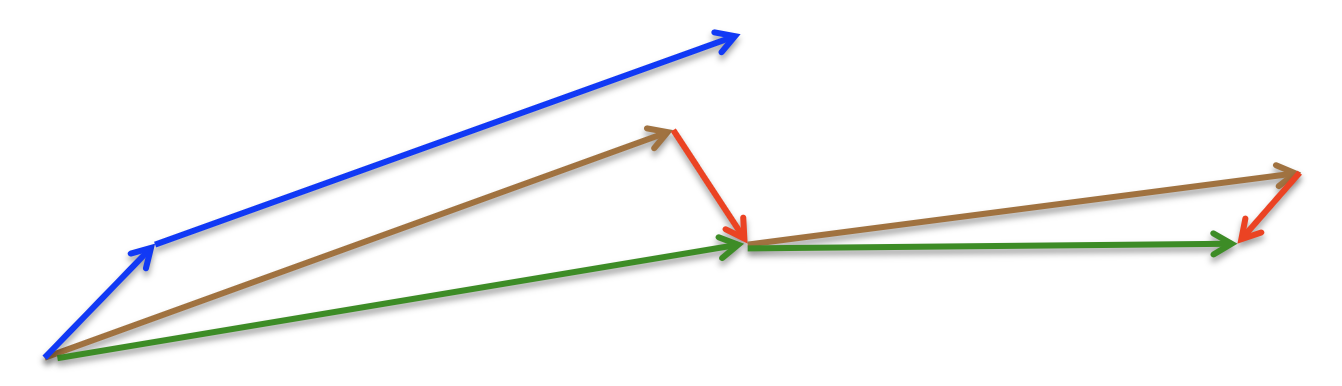
\includegraphics[scale=0.5]{media/hinton_nesterov_momentum.png}
	\caption{
		\parencite[lecture 6c]{hintonNeuralNetworksMachine2012} The blue arrow
		illustrates the movement of heavy ball momentum, i.e. first the small
		``gradient move'', then the large ``momentum move''. Meanwhile the brown
		arrow represents the ``momentum move'' and the red arrow the ``gradient
		move'' for Nesterov's momentum in green. The gradient turns around as we
		move towards the right, and we see that Nesterov's momentum adjusts
		quicker than heavy ball momentum, which is flung outwards.
	}
\end{figure}
%
\begin{definition}[Nesterov's Momentum]
	\label{def: nesterov's momentum}
	\begin{subequations}
	\begin{align}
		\weights_{n+1} &= \weights_n + \lr \momentum_{n+1} \label{eq: nesterov momentum move}\\
		\momentum_{n+1}
		&= (1-\lr\friction)\momentum_n
		- \lr\nabla L[\weights_n + \lr(1-\lr\friction)\momentum_n]
		\label{eq: nesterov momentum}
		\\ \nonumber
		&= \momCoeff\momentum_n
		- \lr\nabla L[\underbrace{
			\weights_n + \momCoeff(\weights_n - \weights_{n-1})
		}_{= y_{n+1}}]
	\end{align}
	\end{subequations}
	%
	Discarding the momentum term and solely using the intermediate position
	results in the simplified version
	%
	\begin{subequations} \label{eq: nesterov intermediate position version}
	\begin{align}
		\weights_{n+1} &= y_{n+1} - \lrSq \nabla \Loss(y_{n+1})\\
		y_{n+1}&= \weights_n + \momCoeff(\weights_n - \weights_{n-1})
	\end{align}
	\end{subequations}
	dropping the intermediate position as well results in the analog to (\ref{eq:
	flat momentum})
	\begin{align}
		\weights_{n+1} &= \weights_n + \momCoeff(\weights_n - \weights_{n-1})
		- \lrSq \nabla \Loss(\weights_n + \momCoeff(\weights_n - \weights_{n-1}))
	\end{align}
\end{definition}
%
\begin{remark}\fxwarning{too informal?}
	This method also known as ``Nesterov's Accelerated Gradient'' (NAG) is said
	to date back to \textcite{nesterovMethodSolvingConvex1983}.  But not only is
	the original text in Russian, it also difficult to find on the internet.
	Fortunately, \citeauthor{nesterovMethodSolvingConvex1983} wrote textbooks,
	\citetitle{nesterovLecturesConvexOptimization2018}
	(\citeyear{nesterovLecturesConvexOptimization2018}) being the most recent.
	Unfortunately Chapter 2.2 on optimal methods provides barely any
	intuition at all, and it is advisable to consult other sources (e.g.
	\textcite{dontlooWhatDifferenceMomentum2016}). Section~\ref{sec: nesterov
	momentum convergence} is an attempt to make these proofs somewhat intuitive.
 \end{remark}

\section{Heavy Ball Convergence}\label{sec: heavy ball convergence}

Following the arguments from Section~\ref{sec: visualize gd} in particular
(\ref{eq: hesse representation of gradient}) we can rewrite the momentum
method as
\begin{align*}
	\begin{pmatrix}
		\weights_n - \hat{\weights}_n \\
		\weights_{n+1} - \hat{\weights}_n
	\end{pmatrix}
	&=
	\begin{pmatrix}
		\weights_n - \hat{\weights}_n \\
		\weights_n - \hat{\weights}_n + \momCoeff (\weights_n - \weights_{n-1})
		- \lrSq \nabla\Loss^2(\weights_n)(\weights_n -\hat{\weights}_n)
	\end{pmatrix}\\
	&=
	\begin{pmatrix}
		0\identity_\dimension & \identity_\dimension \\
		-\momCoeff\identity_\dimension
		& (1+\momCoeff)\identity_\dimension -\lrSq \nabla^2\Loss(\weights_n)
	\end{pmatrix}
	\begin{pmatrix}
		\weights_{n-1} - \hat{\weights}_n \\
		\weights_n - \hat{\weights}_n
	\end{pmatrix}
\end{align*}
%
For readability I will now omit the identity matrix \(\identity\) from the
block matrices which are just a constant multiplied by an identity matrix.
Using the digitalization of the hesse matrix (\ref{eq: diagnalization of the
Hesse matrix}) again, we get
%
\begin{align*}
	&\begin{pmatrix}
		0 & 1 \\
		-\momCoeff & 1+\momCoeff -\lrSq \nabla^2\Loss(\weights_n)
	\end{pmatrix}\\
	&=
	\begin{pmatrix}
		V & 0 \\
		0 & V
	\end{pmatrix}	
	\begin{pmatrix}
		0 & 1 \\
		-\momCoeff &
		\diag(1+\momCoeff -\lrSq\hesseEV_1, \dots, 
		1+\momCoeff -\lrSq\hesseEV_\dimension)
	\end{pmatrix}
	\begin{pmatrix}
		V & 0 \\
		0 & V
	\end{pmatrix}^T
\end{align*}
%
Reordering the eigenvalues to
%
\begin{align*}
	\begin{pmatrix}
		v_1 & 0 & \cdots & v_\dimension & 0 \\
		0 & v_1 & \cdots & 0 & v_\dimension
	\end{pmatrix}
\end{align*}
%
reorders the transformation matrix of the eigenspace to
%
\begin{align}\label{eq: eigenspace momentum transformation}
	\momMatrix := \begin{pmatrix}
		0 & 1 \\
		-\momCoeff & 1+\momCoeff - \lrSq\hesseEV_1 & \\
		& & \ddots & \\
		& & & 0 & 1 \\
		& & & -\momCoeff & 1+\momCoeff - \lrSq\hesseEV_\dimension \\
	\end{pmatrix}
	= \begin{pmatrix}
		\momMatrix_1 \\
		& \ddots\\
		&& \momMatrix_\dimension
	\end{pmatrix}
\end{align}
%
So in contrast to Section~\ref{sec: visualize gd} we do not get a diagonal
matrix immediately. To achieve a similar eigenvalue analysis as in
Section~\ref{sec: visualize gd} we first have to determine the eigenvalues
\(\momEV_{i1},\momEV_{i2}\) of each \(\momMatrix_i\) and then ensure that
\begin{align}
	\max_{i=1,\dots, \dimension} \max\{|\momEV_{i1}|,|\momEV_{i2}|\} < 1.
\end{align}
Using the p-q formula on the characteristic polynomial of \(\momMatrix_i\)
results in 
\begin{align*}
	\momEV_{i1/2}
	= \tfrac12 \left(
		1+\momCoeff-\lrSq\hesseEV_i
		\pm \sqrt{(1+\momCoeff-\lrSq\hesseEV_i)^2 - 4\momCoeff}
	\right).
\end{align*}
%
The analysis of these eigenvalues is very technical and can be found in the
appendix. We will only cover the result here.

\begin{figure}[h]
	\centering
	\def\svgwidth{1\textwidth}
	\input{media/annotated_heavy_ball_rates.pdf_tex}
	\caption{
		Heat plot of \(\max\{|\momEV_1|,|\momEV_2|\}\) for the Heavy Ball Momentum.
		Strictly speaking the ``Monotonic'' (M) and ``Oscillation'' (O) areas should not
		extend into negative \(\momCoeff\) since \(\momEV_{1/2}\)
		have opposite signs there, but it still describes the behavior of the
		dominating eigenvalue. The third label in the legend corresponds to the
		remarkably sharp border of the ``Ripples'' area which I did not want to
		draw over. Also recall that \(\momCoeff=0\) represents SGD
		without momentum.
	}
	\label{fig: annotated heavy ball rates}
\end{figure}

\begin{theorem}[\cite{qianMomentumTermGradient1999}]
	\label{thm: momentum - stable set of parameters}
	Let
	\begin{align*}
		\momEV_{1/2}
		= \tfrac12 \left(
			1+\momCoeff-\lrSq\hesseEV \pm \sqrt{(1+\momCoeff-\lrSq\hesseEV)^2 - 4\momCoeff}
		\right)
	\end{align*}
	then 
	\begin{enumerate}
		\item \(\max\{|\momEV_1|,|\momEV_2|\}<1\) if and only if
		\begin{align*}
			0<\lrSq\hesseEV < 2(1+\momCoeff) \qquad \text{and} \qquad |\momCoeff|<1
		\end{align*}
		\item The complex case can be characterized by either
		\begin{align*}
			0<(1-\sqrt{\lrSq\hesseEV})^2 < \momCoeff < 1
		\end{align*}		
		or alternatively \(\momCoeff>0\) and
		\begin{align*}
			(1-\sqrt{\momCoeff})^2 < \lrSq\hesseEV < (1+\sqrt{\momCoeff})^2,
		\end{align*}
		for which we have \(|\momEV_1|=|\momEV_2|=\sqrt{\momCoeff}\).
		
		As complex
		eigenvalues imply a rotation, this can be viewed as rotating the distance
		to the minimum of the quadratic function into the momentum and back like 
		a pendulum where the friction causes it to eventually end up in the
		minimum. Looking at the distance to the minimum only, we will therefore
		observe a sinus wave (``Ripples'') as the potential energy is transferred
		into velocity and back. In this high momentum case convergence depends
		only on the amount of energy we dissipate through friction and the rate is
		thus equal to the square root of the momentum coefficient \(\beta\)
		regardless of the curvature of the eigenspace.
		\item In the real case we have \(\momEV_1>\momEV_2\) and
		\begin{align}
			\max\{|\momEV_1|, |\momEV_2|\} = \begin{cases}
				|\momEV_1|=\momEV_1 & \lrSq\hesseEV < 1+\momCoeff \\
				|\momEV_2|=-\momEV_2 & \lrSq\hesseEV \ge 1+\momCoeff.
			\end{cases}
		\end{align}
		Restricted to \(1>\momCoeff>0\) this results in two different	
		behaviors. For
		\begin{align*}
			0<\lrSq\hesseEV \le (1-\sqrt{\momCoeff})^2 < 1+\momCoeff
		\end{align*}
		we have \(1>\momEV_1 > \momEV_2 > 0\) which results in a monotonic
		linear convergence (``Monotonic'' case). For
		\begin{align*}
			1+\momCoeff < (1+\sqrt{\momCoeff})^2\le \lrSq\hesseEV < 2(1+\momCoeff)
		\end{align*}
		on the other hand, we get \(-1 < \momEV_2 < \momEV_1 < 0\) which implies 
		an oscillating convergence (``Oscillation''). In contrast to the ``Ripples''
		we switch the side of the distance to the minimum in every iteration.
	\end{enumerate}
\end{theorem}
\begin{proof}
	Appendix Theorem~\ref{thm-appdx: momentum - stable set of parameters}
\end{proof}

In particular (positive) momentum extends the available range for convergent
learning rate/eigenvalue products which allows for larger learning rates. As
can be seen very well in Figure~\ref{fig: annotated heavy ball rates}, the
wider attraction area allows for moving out the largest eigenvalues to the
right with larger eigenvalues shifting the smaller eigenvalues towards the
right as well into more acceptable convergence rates. If the smallest and
largest eigenvalue are far apart (i.e. the condition number \(\condition\) is
high) this should be very useful.

So how much do we gain? In other words what are the optimal rates of
convergence? 

\begin{lemma}[Optimal Parameter Selection]
	\label{lem: optimal hb parameter selection}
	For a given learning rate we have
	\begin{align*}
		\min_{\momCoeff}\max_{i=1,\dots, \dimension}\{|\momEV_{i1}|,|\momEV_{i2}|\}
		= \max\{(1-\sqrt{\lrSq\hesseEV_1}), (1-\sqrt{\lrSq\hesseEV_\dimension})\}
	\end{align*}
	with 
	\begin{align*}
		\arg\min_{\momCoeff}\max_{i=1,\dots,\dimension}\{|\momEV_{i1}|,|\momEV_{i2}|\}
		= \max\{(1-\sqrt{\lrSq\hesseEV_1})^2, (1-\sqrt{\lrSq\hesseEV_\dimension})^2\}
	\end{align*}
	Optimizing over the learning rate \(\lrSq\) as well we get the optimal rate
	\begin{align*}
		\sqrt{\momCoeff_*} = 1-\frac{2}{1+\sqrt{\kappa}}.
	\end{align*}
	for parameters
	\begin{align*}
		\lr_* = \sqrt{\lrSq_*} = \frac{2}{\sqrt{\hesseEV_1}+\sqrt{\hesseEV_\dimension}}
		\qquad
		\momCoeff_*=\left(1-\frac{2}{1+\sqrt{\kappa}}\right)^2
	\end{align*}
\end{lemma}

\begin{proof}
	Since the plot looks quite symmetric it is quite intuitive that
	we only have to consider the largest and smallest eigenvalue. For now we
	can consider it as a lower bound:
	\begin{align}\label{eq: lower bound best heavy ball rates}
		\min_{\momCoeff}\max_{i=1,\dots,\dimension}\{|\momEV_{i1}|,|\momEV_{i2}|\}
		\ge \min_{\momCoeff}
		\max_{i=1,\dimension}\{|\momEV_{i1}|,|\momEV_{i2}|\}
	\end{align}
	Let us inspect the claim
	\begin{align}\label{eq: optimal heavy ball momentum - ev representation}
		\arg\min_{\momCoeff}\max_{i=1,\dimension}\{|\momEV_{i1}|,|\momEV_{i2}|\}
		= \max\{(1-\sqrt{\lrSq\hesseEV_1})^2, (1-\sqrt{\lrSq\hesseEV_\dimension})^2\}
	\end{align}
	In that case we are still (barely) in the complex case, therefore the rate
	of convergence is equal to \(\sqrt{\momCoeff}\), i.e.
	\begin{align*}
		\min_{\momCoeff}\max_{i=1,\dimension}\{|\momEV_{i1}|,|\momEV_{i2}|\}
		= \max\{(1-\sqrt{\lrSq\hesseEV_1}), (1-\sqrt{\lrSq\hesseEV_\dimension})\}
	\end{align*}
	Now let us wiggle around \(\momCoeff\) a bit. If we would increase it, then
	we are obviously increasing our rate since it is then still equal to
	\(\sqrt{\momCoeff}\) as we just expanded the size of the complex case. Now the
	question is what happens if we decrease it. Now by our selection of \(\momCoeff\)
	either the smallest or largest eigenvalue sits right at the edge of the real 
	case. If we can show that our absolute eigenvalue maximum is increasing if
	we move further into the real case (decrease \(\momCoeff\)), we would have
	proven that we can only become worse off doing so. This is annoyingly technical,
	so it is covered in Lemma~\ref{lem-appdx: just at the border of complex case is
	best beta} in the appendix.

	Now since both the largest and smallest eigenvalue are included in the complex
	case, we know that all eigenvalues in between must also be in the complex case
	which means that (\ref{eq: lower bound best heavy ball rates}) is an equality
	proving the first two claims.

	Now we have to optimize over the learning rate \(\lrSq\). Doing our balancing
	act again, only with \(\sqrt{\hesseEV_1},\sqrt{\hesseEV_\dimension}\) instead
	of \(\hesseEV_1,\hesseEV_\dimension\) we get the same result as in
	(\ref{eq: optimal SGD lr eigenvalue representation}), i.e.
	\begin{align*}
		\lr_* = \sqrt{\lrSq_*} = \frac{2}{\sqrt{\hesseEV_1}+\sqrt{\hesseEV_\dimension}}
	\end{align*}
	%
	Since this makes both of them equally bad. We can plug this learning rate into
	either equation from (\ref{eq: optimal heavy ball momentum - ev representation})
	to get the remaining claims about the optimal momentum \(\momCoeff_*\) and optimal
	convergence rate \(\sqrt{\momCoeff_*}\).
\end{proof}

And this convergence rate is in fact \emph{equal} to our lower bound  in
Theorem~\ref{thm: strong convexity complexity bound} (not even up to a
constant!). So on quadratic functions we can not do any better without violating
our assumptions about possible optimizing algorithms (Assumption~ \ref{assmpt:
parameter in generalized linear hull of gradients}).

\section{From Spectral Radius to Operator Norm}

As the Hessian is symmetric the matrix,
\begin{align*}
	1-\lr \nabla^2\Loss
\end{align*}
is symmetric as well. And since we can find an orthonormal basis \((v_1,\dots,
v_\dimension)\) which diagonalizes the matrix, the operator norm is equal
to the spectral radius
\begin{align*}
	\rho(A)
	:= \max_{i=1,\dots,\dimension} |\hesseEV_i|,
\end{align*}
for eigenvalues \(\hesseEV_i\) of matrix \(A\), because of
\begin{align*}
	\|A\| = \sup_{\|x\| =1} \|Ax\|
	= \sup_{\|x\| =1} \sqrt{\langle Ax, Ax\rangle}
	= \sup_{\|x\| =1} \sqrt{\sum_{i=1}^\dimension \hesseEV_i^2 x_i^2},
	= \rho(A)
\end{align*}
where \(x=\sum_{k=1}^\dimension x_i v_i\). The eigenvalue analysis was therefore
sufficient for the gradient descent case. In the momentum case on the other
hand our transformation matrix \(R\) (\ref{eq: eigenspace momentum transformation})
is not symmetric. But the eigenvalue analysis is still useful due to Gelfand's Formula
\parencite{gelfandNormierteRinge1941} i.e.
\begin{align*}
	\rho(R) = \lim_{n\to\infty}\sqrt[n]{\|R^n\|}
\end{align*}
This formula is used by \textcite[p. 38, Lemma 1]{polyakIntroductionOptimization1987}
to argue, that we have for all \(\epsilon>0\)
\begin{align*}
	\|R^n\|\le \text{const } (\rho(R) + \epsilon)^n.
\end{align*}
This still provides exponential convergence to zero for any spectral radius
\(\rho(R)\) smaller one. Therefore the eigenvalue analysis is still useful.

\textcite{kozyakinAccuracyApproximationSpectral2009} already provides much tighter
bounds with more explicit constants, but they still depend on the unknown quantity
\begin{align*}
	\max_{i=1,\dots,\dimension}\frac{\|R_i^2\|}{\|R_i\|^2}.
\end{align*}
Where we can use their bounds for two dimensional matrices as the orthogonality
argument still applies between blocks, so we can consider the operator norm of
one block and take the maximum over all blocks
\begin{align*}
	\|R\| = \max_{i=1,\dots,\dimension}\|R_i\|
	= \max_{i=1,\dots,\dimension}\left\|
	\begin{pmatrix}
		0 & 1 \\
		-\momCoeff & 1+\momCoeff-\lrSq\hesseEV_i
	\end{pmatrix}
	\right\|.
\end{align*}

\subsection{Actually Explicit Bounds}

To build some intuition, notice how \(\lrSq\hesseEV_i=1\) and \(\momCoeff=1\)
lead to
\begin{align*}
	R_i
	=\begin{pmatrix}
		0 & 1 \\
		0 & 0
	\end{pmatrix}
\end{align*}
of which both eigenvalues are zero, but the operator norm is one as the vector
\((0, 1)^T\) does not change in length. Notice how we simply move the more
recent weight up into the older weight slot. If we would apply the matrix again
our weights would fully disappear. In other words: The problem are the cyclical
eigenspaces, in the jordan normal form. More precisely, we can find some
basis change \(U\) such that
\begin{align*}
	R_i^n
	= \left(U 
		\begin{pmatrix}
			r_{i1} & \delta\\
			0 & r_{i2}
		\end{pmatrix}
	U^{-1}\right)^n
	= U 
	\begin{pmatrix}
		r_{i1} & \delta\\
		0 & r_{i2}
	\end{pmatrix}^n
	 U^{-1}
\end{align*}
where \(\delta\) is zero when \(r_{i1}\neq r_{i2}\) and can be zero or one if
they are equal. Now if they are both equal to some value \(r_i\), then we
can write
\begin{align*}
	\begin{pmatrix}
		r_i & \delta\\
		0 & r_i
	\end{pmatrix}^n
	&= \left(r_i\identity + 
	\begin{pmatrix}
		0 & \delta\\
		0 & 0 
	\end{pmatrix}\right)^n
	= \sum_{k=0}^n \binom{n}{k} r_i^k \begin{pmatrix}
		0 & \delta \\
		0 & 0
	\end{pmatrix}^{n-k}\\
	&= r_i^n\identity + n r_i^{n-1}\begin{pmatrix}
		0 & \delta \\
		0 & 0
	\end{pmatrix}
	= \begin{pmatrix}
		r_i^n & \delta n r_i^{n-1} \\
		0 & r_i^n
	\end{pmatrix}.
\end{align*}
So together with the case \(\delta=0\), we get
\begin{align*}
	R_i^n = U\begin{pmatrix}
		r_{i1}^n & \delta n r_{i1}^n\\
		0 & r_{i2}^n
	\end{pmatrix}U^{-1},
\end{align*}
Which results in
\begin{align*}
	\|R_i^n\|
	&\le \|U\|
	\left\| \begin{pmatrix}
		r_{i1}^n & \delta n r_{i1}^{n-1}\\
		0 & r_{i2}^n
	\end{pmatrix} \right\|
	\|U^{-1}\|\\
	&\le \|U\|\|U^{-1}\|
	\left(
	\left\| \begin{pmatrix}
		r_{i1}^n & 0\\
		0 & r_{i2}^n
	\end{pmatrix} \right\|
	+ \delta
	\left\| \begin{pmatrix}
		0 &  n r_{i1}^{n-1}\\
		0 & 0
	\end{pmatrix} \right\|
	\right)\\
	&= \|U\|\|U^{-1}\| (\rho(R_i)^n+ \delta n |r_{i1}|^{n-1})\\
	&= \|U\|\|U^{-1}\| (\rho(R_i)+ \delta n)\rho(R_i)^{n-1}\\
	&\in O(n\rho(R_i)^{n}) \subset O((\rho(R_i)+\epsilon)^n).
\end{align*}
%
Of course we do not have any bounds for \(\|U\|\|U^{-1}\|\) so this is still
not explicit enough. And the fact that \(\delta\) jumps from zero to one once the
eigenvalues are not equal anymore does not inspire confidence in the continuity
of \(U\). In fact \textcite[Section 7.1.5]{golubMatrixComputations2013} claim
that ``any matrix [...] that diagonalizes
\begin{align*}
	\begin{pmatrix}
		1+\epsilon & 1 \\
		0 & 1-\epsilon
	\end{pmatrix},
	\qquad \epsilon \ll 1,
\end{align*}
has a 2-norm condition of order \(1/\epsilon\)''. Now this is not the same matrix
but this example shows that we have to be careful. Especially since we try to select
our learning rate \(\lrSq\) and momentum coefficient \(\momCoeff\) in such a way
that we are right on the complex border (Lemma~\ref{lem: optimal hb parameter
selection}). So we do in fact strive for the term inside the square root to be zero
\begin{align*}
	\momEV_{i1/2}
	= \tfrac12 \left(
		1+\momCoeff-\lrSq\hesseEV_i
		\pm \sqrt{(1+\momCoeff-\lrSq\hesseEV_i)^2 - 4\momCoeff}
	\right),
\end{align*}
and should therefore assume to be very close to \(r_{i1}=r_{i2}\).

Instead of the Jordan Normal form, we therefore want to use a numerically more
stable transformation, the ``Schur decomposition''.

\subsubsection{Schur Decomposition}

\begin{theorem}[Schur decomposition, {\cite[Theorem 7.1.3]{golubMatrixComputations2013}}]
	If \(A\in\complex^{\dimension\times \dimension}\), then there exists a unitary
	\(Q\in\complex^{\dimension\times \dimension}\) such that
	\begin{align*}
		Q^* A Q = \diag(\hesseEV_1, \dots, \hesseEV_\dimension) + N
	\end{align*}
	where \(N\) is strictly upper triangular and \(Q^*\) is the conjugate
	transpose of \(Q\).
\end{theorem}

The neat thing about this result is that unitary matrices are isometries for the
euclidean norm.

\begin{lemma}[Unitary Matrices are Isometries]
	\label{lem: unitary matrices are isometries}
	Unitary matrices \(Q\) are isometries with regard to the euclidean norm
	\begin{align*}
		\|Qx\|_2 = \|x\|_2 \qquad \forall x\in\complex^\dimension
	\end{align*}	
	and also with regard to the induced operator norm
	\begin{align*}
		\|QA\| = \|A\| \quad \text{and} \quad \|AQ\| = \|A\|
		\qquad \forall A \in\complex^{\dimension\times\dimension}
	\end{align*}
\end{lemma}
\begin{proof}
	It is straightforward to show the isometry on euclidean norms
	\begin{align*}
		\|Qx\|^2 = \langle Qx, Qx\rangle = x^* Q^* Q x = x^* x = \|x\|^2.
	\end{align*}
	This then translates to them being isometries for the induced operator norm
	on matrices, since
	\begin{align*}
		\|QA\| = \sup_{\|x\|=1} \|QAx\| = \sup_{\|x\|=1} \|Ax\|
	\end{align*}
	and
	\begin{align*}
		\|AQ\|
		&= \sup_{x} \frac{\|AQx\|}{\|x\|} = \sup_{x} \frac{\|AQx\|}{\|Qx\|}
		= \sup_{y} \frac{\|Ay\|}{\|y\|} = \|A\|.
		\qedhere
	\end{align*}
\end{proof}

This lemma allows us to completely disregard the basis change matrices  in our
problem of estimating the operator norm of \(R\). And as we are only concerned
with \(2\times 2\) matrices, ``strictly upper triangular'' still means only one
entry. So we can deal with it very similarly as with the jordan normal form. The
only issue is, we need to actually know the entry in the upper right corner to
create an upper bound. But as it turns out, calculating the Schur decomposition
for \(2\times 2\) matrices is very simple. We just need one normalized
eigenvector and (any of the two) normalized vectors in its orthogonal
complement.

\begin{lemma}[Explicit Schur Decomposition for Specific Matrix]
	\label{lem: explicit schur decomposition}
	For a real matrix of the form
	\begin{align*}
		R = \begin{pmatrix}
			0 & 1 \\
			-\momCoeff & \xi
		\end{pmatrix},
	\end{align*}
	the unitary operator	
	\begin{align*}
		Q:=\frac{1}{\sqrt{1+|r_1|^2}} \begin{pmatrix}
		1 & \conjugate{r}_1 \\
		r_1 & -1
	\end{pmatrix}
	\end{align*}
	where
	\(
		r_{1/2}
		= \tfrac12 \left(
			\xi \pm \sqrt{\xi^2 - 4\momCoeff}
		\right)
	\)
	are the eigenvalues of \(R\), results in the Schur Decomposition
	\begin{align*}
		Q^* R Q
		&=\begin{pmatrix}
			r_1
			& -\frac{(1+\momCoeff)(1+\conjugate{r}_1^2)}{1+|r_1|^2} \\
			0 &  \frac{\momCoeff\conjugate{r}_1 + r_2}{1+|r_1|^2}
		\end{pmatrix}.
	\end{align*}
	For complex eigenvalues, more specifically \(4\momCoeff\ge\xi^2\), we have
	\begin{align*}
		Q^* R Q
		&=\begin{pmatrix}
			r_1
			& -(1+\conjugate{r}_1^2) \\
			0 & \conjugate{r}_1 
		\end{pmatrix}.
	\end{align*}
	Note that \(r_1\) and \(r_2\) could always be swapped to achieve a more favorable result.
\end{lemma}
\begin{proof}
	Since
	\begin{align*}
		\frac{1}{\sqrt{1+|r_1|^2}} \begin{pmatrix}
			1 \\
			r_1
		\end{pmatrix}
	\end{align*}
	is a normalized eigenvector for eigenvalue \(r_1\) of \(R\), there are
	only two options for an orthonormal second vector, which results in \(Q\).

	Recall that any eigenvalue of \(R\), in particular \(r_1\) and
	\(\conjugate{r}_1\in\{r_1, r_2\}\), is a root of the characteristic polynomial
	\begin{align}\label{eq: property of eigenvalues of R}
		\det (r\identity - R) = r^2 - r\xi + \momCoeff = 0.
	\end{align}
	Now we can calculate the Schur decomposition of \(R\):
	\begin{align*}
		Q^* R Q
		&= \frac{1}{1+|r_1|^2} \begin{pmatrix}
			1 & \conjugate{r}_1 \\
			r_{1} & -1
		\end{pmatrix}
		\begin{pmatrix}
			0 & 1 \\
			-\momCoeff & \xi
		\end{pmatrix}
		\begin{pmatrix}
			1 & \conjugate{r}_1 \\
			r_1 & -1
		\end{pmatrix}\\
		&= \frac{1}{1+|r_{1}|^2} \begin{pmatrix}
			1 & \conjugate{r}_1 \\
			r_1 & -1
		\end{pmatrix}
		\begin{pmatrix}
			r_1 & -1 \\
			\smash{\underbrace{-\momCoeff + \xi r_1}_{
				=r_1^2 \ (\ref{eq: property of eigenvalues of R})
			}}
			& -\momCoeff \conjugate{r}_1 - \xi
		\end{pmatrix}
		\vphantom{\underbrace{\begin{pmatrix}1\\1\end{pmatrix}}_{=2}}
		\\
		&=\frac{1}{1+|r_{1}|^2}\begin{pmatrix}
			r_1(1+|r_1|^2)
			& -\momCoeff \conjugate{r}_1^2  + (1+\xi \conjugate{r}_1) \\
			0 &  \momCoeff\conjugate{r}_1 + \xi - r_1
		\end{pmatrix}\\
		&\lxeq{(\ref{eq: property of eigenvalues of R})}\begin{pmatrix}
			r_1
			& -\frac{\momCoeff \conjugate{r}_1^2 + 1+ (\conjugate{r}_1^2 + \momCoeff)}{1+|r_1|^2} \\
			0 &  \frac{\momCoeff\conjugate{r}_1 + \xi - r_1}{1+|r_1|^2}
		\end{pmatrix}\\
		&=\begin{pmatrix}
			r_1
			& -\frac{(1+\momCoeff)(1+\conjugate{r}_1^2)}{1+|r_1|^2} \\
			0 &  \frac{\momCoeff\conjugate{r}_1 + r_2}{1+|r_1|^2}
		\end{pmatrix}
	\end{align*}
	where we have used \(\xi - r_1 = r_2\) in the last equation. Now in the complex
	case (and the case \(4\momCoeff = \xi^2\)) we have
	\(|r_1|=|r_2|=\sqrt{\momCoeff}\) and \(\conjugate{r_1} = r_2\) which results
	in
	\begin{align*}
		Q^* R Q
		&=\begin{pmatrix}
			r_1
			& -(1+\conjugate{r}_1^2) \\
			0 & \conjugate{r}_1 
		\end{pmatrix}.
		\qedhere
	\end{align*}
\end{proof}

\begin{theorem}[Upper Bound on Operator Norm]
	Assuming our momentum coefficient is large enough but smaller one, i.e.
	\begin{align*}
		1>\momCoeff
		\ge \max\{(1-\sqrt{\lrSq\hesseEV_1})^2, (1-\sqrt{\lrSq\hesseEV_\dimension})^2\},
	\end{align*}
	we are in the complex case, i.e. \(\rho(R) = \sqrt{\momCoeff}\) and
	\begin{align*}
		\|R^n\|
		&\le \rho(R)^{n-1}(\rho(R)+n[1+\rho(R)^2])\\
		&\le 3n\rho(R)^{n-1} \qquad \forall n\ge 1.
	\end{align*}
	For all \(\epsilon>0\) we therefore have
	\begin{align*}
		\|R^n\|
		&\le \frac{3\exp(1)/\rho(R)}{\log(\rho(R)+\epsilon)-\log(\rho(R))}
		[\rho(R)+\epsilon]^n
		\\
		&\in O([\rho(R)+\epsilon]^n).
	\end{align*}
\end{theorem}
\begin{proof}
	First we apply our Lemmas to get
	\begin{align*}
		\|R^n\|
		&=\max_{i=1,\dots,\dimension}	\|R_i^n\|
		\xeq{\ref{lem: unitary matrices are isometries},\ \ref{lem: explicit schur decomposition}}
		\max_{i=1,\dots,\dimension}\left\|\begin{pmatrix}
			r_{i1} & -(1+\conjugate{r}_{i1}^2)\\
			0 & \conjugate{r}_{i1}
		\end{pmatrix}^n\right\|.
	\end{align*}
	Then we use Lemma~\ref{lem-appdx: absolute value inside operator norms} to
	turn the entries into their absolute values which makes the diagonal entries
	equal. As the diagonal now commutes with the nilpotent matrix we can apply the
	binomial theorem 
	\begin{align*}
		\|R^n\|
		&\le \max_{i=1,\dots,\dimension}
		\Bigg\|\left(
		\begin{pmatrix}
			|r_{i1}| & 0\\
			0 & |r_{i1}|
		\end{pmatrix}
		+ \begin{pmatrix}
			0 & |1+\conjugate{r}_{i1}^2|\\
			0 & 0
		\end{pmatrix}
		\right)^n\Bigg\|\\
		&\le \max_{i=1,\dots,\dimension}
		\Bigg\|
		\sum_{k=0}^n \binom{n}{k}
				|r_{i1}|^{n-k}
			\underbrace{
				\left(
				|1+\conjugate{r}_{i1}^2|
				\begin{pmatrix}
					0 & 1\\
					0 & 0
				\end{pmatrix}
				\right)^k
			}_{=0 \ \forall k>1}
		\Bigg\|\\
		&\le \max_{i=1,\dots,\dimension}
		|r_{i1}|^n \|\identity\| + n |r_{i1}|^{n-1}(|1|+|r_{i1}^2|)
		\underbrace{
			\Bigg\|
				\begin{pmatrix}
					0 & 1\\
					0 & 0
				\end{pmatrix}
			\Bigg\|
		}_{=1}
		\\
		&\le \max_{i=1,\dots,\dimension}
		\rho(R_i)^n + n \rho(R_i)^{n-1}(1+\rho(R_i)^2)\\
		&=	\rho(R)^{n-1}(\rho(R) + n [1+\rho(R)^2]).
	\end{align*}
	For the second claim let \(\epsilon>0\), then we have
	\begin{align*}
		\frac{\|R^n\|}{[\rho(R)+\epsilon]^n}
		&\le \frac{3n\rho(R)^{n-1}}{[\rho(R)+\epsilon]^n}\\
		&= \frac{3}{\rho(R)}\exp(\log(n) + n[\log(\rho(R))-\log(\rho(R)+\epsilon)])\\
		&\le \frac{3}{\rho(R)}\exp
		\left(\log\left(\frac{1}{[\log(\rho(R)+\epsilon)-\log(\rho(R))]}\right) + 1\right)\\
		&= \frac{3\exp(1)/\rho(R)}{\log(\rho(R)+\epsilon)-\log(\rho(R))}.
	\end{align*}
	Here we simply maximized over \(n\) to obtain the last inequality.
\end{proof}


\section{Why Consider Alternatives?}

Now while Nesterov's Momentum breaks Assumption~\ref{assmpt: parameter in
generalized linear hull of gradients} as it uses gradients at a
different point than the iterates, it does not break it fundamentally. The
assumption applies to the intermediate states \(y_n\) which are not too far
from our actual iterates and would thus allow us to make similar statements
about them with a bit of work.

And while Heavy Ball Momentum can already almost achieve the optimal convergence
rate of our complexity bounds up to some issues with the operator norm, there
are more issues with it besides this particular sticking point.

\subsubsection{Weakest Link Contraction Factor}

The first issue you
might have noticed is: Since \emph{all eigenspaces} are in the complex case,
all of them have the worst contraction factor \(\sqrt{\momCoeff_*}\). In stochastic
gradient descent on the other hand the contraction factor is \(|1-\lr_*\hesseEV_i|\)
for the eigenspace \(i\), which can be considerably better than the worst
contraction factor 
\[|1-\lr_*\hesseEV_\dimension|=|1-\lr_*\hesseEV_1|.\]
To improve the convergence rates of the worst eigenspaces we have therefore
sacrificed the (possibly excellent) convergence rates of all other eigenspaces.

\subsubsection{No General Convergence at these Rates}

While
\textcite[pp. 65-67]{polyakIntroductionOptimization1987} used the eigenvalue
analysis of \(\nabla\Loss^2(\weights_*)\) to extend this rate of convergence
to a local area around \(\weights_*\), \textcite[pp. 78-79]{lessardAnalysisDesignOptimization2016}
gave an example of an \(\strongConvex{\lbound}{\ubound}\) function where
the heavy ball method with these ``optimal'' parameters is trapped in an attractive
cycle instead of converging. 
%
\begin{figure}[h]
	\centering
	\def\svgwidth{1\textwidth}
	\input{media/hb_counterexample.pdf_tex}
	\caption{
		\citeauthor{lessardAnalysisDesignOptimization2016}'s counterexample.
		Notice that the y-axis is much coarser than the x-axis and gradients are
		therefore much steeper than apparent. At point \(-1.8\) the gradient is
		quite steep and the next parameter is flung across the minimum to
		\(2.12\). Due to the less convex segment on this side, the gradient is
		not quite as steep here, so the iterate does not make it to the other
		side again which would then cause a bouncing back and forth to the
		minimum. Instead it stays on this side, which causes the next gradient
		at \(0.65\) together with the built momentum in this direction to move the
		iterate back out to our first point.
	}
	\label{fig: heavy ball counterexample}
\end{figure}

Since we know \(\lbound\) and \(\ubound\) of their counterexample function from
Figure~\ref{fig: heavy ball counterexample}, we know the parameters \(\lrSq_*\)
and \(\momCoeff_*\) which they used to explicitly write out the momentum recursion
with \(\weights_{n+1}, \weights_{n}, \weights_{n-1}\). Assuming a three-cycle
this left them with just three linear equations which results in the three-cycle
displayed in the Figure. Since we start with zero momentum, we just have to
find a point to enter this cycle. Additional to solving this initialization
problem, \textcite[pp. 93-94]{lessardAnalysisDesignOptimization2016} also show
that this cycle is stable under noise (attractive).

\textcite{ghadimiGlobalConvergenceHeavyball2015} salvages some of this wreckage
by proving general convergence results with tighter restrictions on hyper
parameters. In particular for \(\Loss\in\strongConvex{\lbound}{\ubound}\) and
\begin{align*}
	\momCoeff\in[0,1),
	\qquad \lrSq\in \left(0, \frac{2(1-\momCoeff)}{\ubound+\lbound}\right)
\end{align*}
they can guarantee linear convergence with an explicit, but complicated
\fxnote{take a closer look?}{contraction factor}. Notice that this is
considerably weaker than the condition
\begin{align*}
	0<\lrSq\lbound \le \dots \le \lrSq\ubound < 2(1+\momCoeff)
\end{align*}
from Theorem~\ref{thm: momentum - stable set of parameters}. In particular
momentum stops increasing the selection space for learning rates, just like
\(\lbound\) which rules out our optimal parameters immediately. 

Similarly they prove that for \(\Loss\in\lipGradientSet{\ubound}\) and
\begin{align*}
	\momCoeff\in[0,1),
	\qquad \lrSq\in \left(0, \frac{(1-\momCoeff)}{\ubound}\right]
\end{align*}
that the running minimum of loss evaluation converges to the minimal loss,
with their best guarantee achieved for \(\lrSq =(1-\momCoeff)/\ubound\)
resulting in
\begin{align*}
	\min_{k=0,\dots,n}\Loss(\weights_k) -\Loss(\weights_*)
	\le \frac{1}{1-\momCoeff}\frac{\ubound\|\weights_0-\weights_*\|^2}{2(n+1)}
\end{align*}
which provides a tighter convergence bound than 
Theorem~\ref{thm: convex function GD loss upper bound} for gradient descent 
without momentum \(\momCoeff=0\), but is actually harmed by momentum. While
this bound might not be the best and further improvements could be made
\parencite[see e.g.][]{sunNonErgodicConvergenceAnalysis2019} it appears that we
always end up with \(O(1/n)\) convergence rates in the general case and we
therefore turn towards Nesterov's Momentum.

\section{Nesterov's Momentum Convergence}\label{sec: nesterov momentum convergence}

The Eigenvalue analysis of Nesterov's Momentum starts out very similar and we
easily obtain the analog eigenspace transformation to (\ref{eq: eigenspace
momentum transformation})
%
\begin{align*}
	\momMatrix_i = \begin{pmatrix}
		0 & 1\\
		-\momCoeff(1-\lrSq\hesseEV_i) & (1+\momCoeff)(1-\lrSq\hesseEV_i).
	\end{pmatrix}	
\end{align*}
%
which curiously reduces to the heavy ball version if we use
\begin{align}\label{eq: tilde momentum}
	\tilde{\momCoeff}_i = \momCoeff(1-\lrSq\hesseEV_i)
\end{align}
We therefore immediately get from Theorem~\ref{thm: momentum - stable set of
parameters} that \(\max\{|\momEV_{i1}|,|\momEV_{i2}|\}<1\) if and only if
\begin{align*}
	0<\lrSq\hesseEV_i < 2(1+\tilde{\momCoeff}_i)
	\quad \text{and} \quad
	|\tilde{\momCoeff}_i|<1
\end{align*}
%
which after some transformations is itself equivalent to
\begin{align*}
	0<\lrSq\hesseEV_i < 1+\frac{1}{1+2\momCoeff}
	\quad \text{and} \quad
	|1-\lrSq\hesseEV_i|<\frac{1}{|\momCoeff|}.
\end{align*}
%
\begin{figure}[h]
	\centering
	\def\svgwidth{1\textwidth}
	\input{media/annotated_nesterov_rates.pdf_tex}
	\caption{
		Heat plot of \(\max\{|\momEV_1|,|\momEV_2|\}\) for the Nesterov Momentum.
		``M'' and ``O'' stand for the ``Monotonic'' and ``Oscillating'' types of 
		real eigenvalues. Note that the separating line of these cases
		\(\lrSq\hesseEV=1+\tilde{\momCoeff}=1+\momCoeff(1-\lrSq\hesseEV)\)
		reduces to \(\lrSq\hesseEV=1\) but since we divide by \(1+\momCoeff\)
		the sides flip at \(\momCoeff=-1\). Again the third label is omitted to
		keep the remarkably sharp border unobstructed.
	}
	\label{fig: annotated nesterov rates}
\end{figure}

In a sense Nesterov's Momentum provides every eigenspace with its own
heavy ball momentum \(\tilde{\momCoeff}_i\) which is a good sign if we want
to avoid the ``Weakest Link Contraction Factor'' issue we had in heavy ball
momentum. And if we are in the complex case the convergence rate is
\(\sqrt{\momCoeff(1-\lrSq\hesseEV_i)}\) which looks like the root of the
gradient descent convergence rate multiplied by a factor we could make smaller
than one.

As we have reduced our problem to the heavy ball problem again, we can also use
the same arguments to bound the operator norm. We will therefore ignore that
problem henceforth.

To ensure all eigenspaces are in the complex case, we first need to ensure that
all \(\tilde{\momCoeff}_i\) are positive which requires
\begin{align*}
	1-\lrSq\hesseEV_i >= 0
\end{align*}
So let us select \(\lrSq= 1/\hesseEV_\dimension\). Now we just need to ensure
that the smallest eigenvalue is in the complex case, for that set it to be
right on the border \(\tilde{\momCoeff}_1=(1-\sqrt{\lrSq\hesseEV_1})^2\),
which then results in
\begin{align*}
	\momCoeff = \frac{(1-\sqrt{\lrSq\hesseEV_1})^2}{1-\lrSq\hesseEV_1}
	=\frac{1-\sqrt{\lrSq\hesseEV_1}}{1+\sqrt{\lrSq\hesseEV_1}}
	=\frac{1-\sqrt{1/\condition}}{1+\sqrt{1/\condition}} (< 1).
\end{align*}
Since
\begin{align*}
	\tilde{\momCoeff}_1 >= \dots >=\tilde{\momCoeff}_\dimension=0
\end{align*}
the worst rate convergence is exhibited by the first eigenspace and is equal to
\begin{align}\label{eq: nesterov convegence rate eigenvalue derivation}
	\sqrt{\tilde{\momCoeff}_1} = \sqrt{(1-\sqrt{\lrSq\hesseEV_1})^2}
	= 1-\sqrt{1/\condition} = 1- \frac{1}{\sqrt{\condition}}.
\end{align}
%
This rate of convergence is a tiny bit worse than the optimal heavy ball
convergence rate \(1-2/(1+\sqrt{\condition})\), which is also the complexity
bound, but it is quite similar.

Now if you had a look at Figure~\ref{fig:
annotated nesterov rates} you might have noticed that for a fixed learning
rate the \(\lrSq\hesseEV_i\) are \(\dimension\) vertical lines. We made sure
that the rightmost line was right on top of the black line and then moved up
our momentum term until all our rates where in the ripples area. From the
plot you might get the intuition that we can improve convergence if we
increase the learning rate to move the largest eigenvalue into the oscillating
range just like in the gradient descent. And this is in fact not the optimal
selection of learning rates. \textcite{lessardAnalysisDesignOptimization2016}
claim\footnote{The proof is left to the reader} that optimal tuning results in
\begin{align*}
	\lrSq = \frac{4}{3\ubound + \lbound}
	\quad \text{and} \quad
	\momCoeff = \frac{\sqrt{3\condition+1}-2}{\sqrt{3\condition+1}+2}
\end{align*}
with learning rate
\begin{align*}
	1-\frac{2}{\sqrt{3\condition+1}}.
\end{align*}
But as we have learned with
Heavy Ball Momentum, optimal learning rates are no use if we can not generalize
them.

\subsection{Estimating Sequences}

To prove convergence for gradient descent we proved that gradient descent
minimizes a ``local'' upper bound (Lemma~\ref{lem: smallest upper bound}). Local
in the sense that we only use the gradient information at our current position
and discard all previous gradient information. To prove better convergence rates
we need to utilize the previous gradients too.

Let us start with an upper bound of the form
%
\begin{align}\label{eq: Phi_0 (upper bound - kinda)}
	\Phi_0(\weights) = \underline{\Phi}_0 + \tfrac{\lbound_0}{2}\|\weights-z_0\|^2.
\end{align}
%
One example for such an upper bound is
%
\begin{align*}
	\weights \mapsto
	\Loss(y_0)
	+ \langle\nabla\Loss(y_0), \weights - y_0\rangle
	+ \tfrac{\ubound}{2}\|\weights -y_0\|^2.
\end{align*}
%
Which can be written as in (\ref{eq: Phi_0 (upper bound - kinda)}) with
\(\lbound_0=\ubound\) by selecting
%
\begin{align*}
	z_0 = y_0 - \ubound^{-1}\nabla\Loss(y_0).
\end{align*}
This is the same technique as we used in (\ref{eq: newton minimum approx}). Keep
in mind that our upper bound is a quadratic function which therefore
is equal to its second taylor derivative.

Now since we started with an upper bound, it is trivial to find \(\weights_0\)
such that
\begin{align*}
	\Loss(\weights_0) \le \min_{\weights}\Phi_0(\weights)
\end{align*}
as we can simply select \(\weights_0=z_0\) to get
\begin{align*}
	\Loss(\weights_0) =\Loss(z_0) \le \Phi_0(z_0) = \min_{\weights}\Phi_0(\weights).
\end{align*}
Now the idea is to morph our upper bound \(\Phi_0\) via \(\Phi_n\) slowly into
a lower bound while keeping 
\begin{align}\label{eq: staying ahead of the estimates}
	\Loss(\weights_n) \le \min_{\weights}\Phi_n(\weights)=:\underline{\Phi}_n.
\end{align}
This would force \(\weights_n\) towards the minimum as it needs to stay smaller
than \(\Phi_n\) which changes into a lower bound of \(\Loss\). By controlling
the speed of morphing we will be able to bound the convergence speed. But we
can not morph too fast otherwise we will not be able to stay ahead of it, i.e.
fulfill (\ref{eq: staying ahead of the estimates}). Okay now that we have set
up the gameplan let us make this more concrete.
The obvious lower bounds we want to utilize are made up of all the gradients we
collect along the way
\begin{align*}
	\phi_n(\weights)
	:= \Loss(y_n) + \langle\nabla\Loss(y_n), \weights-y_n\rangle
	+ \tfrac{\lbound}{2}\|\weights-y_n\|^2.
\end{align*}
where this includes the non strongly convex case with \(\lbound=0\). So let
us consider
\begin{align*}
	\Phi_1 = \gamma \phi_1 + (1-\gamma)\Phi_0
\end{align*}
For \(\gamma=1\) we would have a lower bound, but if \(\nabla\Loss(y_1)\)
does not happen to be zero, the tangent point \(y_1\) is sitting on a slope and
therefore is not smaller than the minimum of \(\phi_1=\Phi_1\) and since \(\phi_1\)
is a lower bound on \(\Loss\) it will generally be impossible to satisfy
(\ref{eq: staying ahead of the estimates}) with \(\weights_1\) in that case.
So the first take-away is, that we can generally not select \(\gamma=1\)
unless we are already in the minimum. But this also hints at another issue:
A convex combination of lower bounds
\begin{align*}
	\sum_{k=0}^n \hat{\gamma}_k \phi_k(\weights)
\end{align*}
is also a lower bound. But since they generally only have one tangent point
which is equal and are otherwise strictly lower, it is difficult to find
a \(\weights\) such that \(\Loss(\weights)\) is smaller than its minimum.
So the \(y_k\) already need to be equal to the minimum
of \(\Loss\) such that the \(\phi_k\) start out with no slope and their
minimum is also equal to \(\weights_*\). If we have
\begin{align*}
	\sum_{k=1}^n \hat{\gamma}_k \phi_k(\weights)
	+ \hat{\gamma}_0 \Phi_0(\weights)
\end{align*}
we get a bit more wiggle room but if we want to slowly remove our upper bound
we run into a similar problem. Therefore we also need to slowly remove the old
\(\phi_k\) upper bounds, constructed with \(y_k\) far away from the minimum
\(\weights_*\). This motivates why we might wish to select
\begin{align}\label{eq: estimating sequence recursion}
	\Phi_n(\weights) := \gamma_n \phi_n(\weights) + (1-\gamma_n)\Phi_{n-1}(\weights)
\end{align}
causing an exponential decay not only for the initial upper bound, but also for
our previous lower bounds. For
\begin{align*}
	\Gamma_k^n := \prod_{i=k}^n (1-\gamma_i)
\end{align*}
one can inductively convert the recursion (\ref{eq: estimating sequence
recursion}) into
\begin{align}
	\nonumber
	\Phi_n(\weights)
	&= \sum_{k=1}^n \Gamma_{k+1}^n\gamma_k \phi_k(\weights)
	+ \Gamma_1^n\Phi_0(\weights) \\
	\label{eq: estimating sequence explicit}
	&\le (1-\Gamma_1^n)\Loss(\weights) + \Gamma_1^n\Phi_0(\weights)
\end{align}

\begin{lemma}
	\label{lem: estimating sequence convergence speed}
	If the \(\weights_n\) satisfy (\ref{eq: staying ahead of the estimates}),
	then we have
	\begin{align*}
		\Loss(\weights_n) - \Loss(\weights_*)
		\le \Gamma_1^n (\Phi_0(\weights_*)-\Loss(\weights_*)).
	\end{align*}
	This motivates why we are interested in \(\Gamma_1^n\to 0\). A sufficient
	condition is
	\begin{align*}
		\sum_{k=0}^\infty \gamma_k = \infty
	\end{align*}
\end{lemma}
\begin{proof}
	Both statements are fairly easy to prove:
	\begin{align*}
		\Loss(\weights_n)
		\xle{(\ref{eq: staying ahead of the estimates})}
		\min_{\weights}\Phi_n(\weights)
		&\lxle{(\ref{eq: estimating sequence explicit})} \min_{\weights} \{
		(1-\Gamma_1^n) \Loss(\weights) + \Gamma_1^n\Phi_n(\weights) \}\\ 
		&\le (1-\Gamma_1^n) \Loss(\weights_*) + \Gamma_1^n\Phi_n(\weights_*)
	\end{align*}
	Subtracting \(\Loss(\weights_*)\) from both sides lets us move on to the
	second statement:
	\begin{align*}
		\Gamma_1^n &= \prod_{i=1}^n (1-\gamma_i)
		\le\prod_{i=1}^n \exp(-\gamma_i)
		= \exp\left(-\sum_{i=1}^n\gamma_i\right) \to 0
		\qedhere
	\end{align*}
\end{proof}

Now we just need to make sure that we can actually satisfy (\ref{eq: staying
ahead of the estimates}) while making \(\gamma_k\) as large as possible.
For that we want an explicit representation of \(\underline{\Phi}_{n}\).
Fortunately we are only adding up quadratic functions therefore the function
\(\Phi_{n}\) is quadratic too and can thus be written in the form
\begin{align}\label{eq: centered Phi representation}
	\Phi_{n}(\weights) = \underline{\Phi}_{n} + \tfrac{\lbound_{n}}{2}\|\weights - z_n\|^2
\end{align}
where our convexity parameter \(\lbound_n\) morphs from \(\lbound_0\) to
\(\lbound\)
\begin{align}\label{eq: lbound recursion}
	\lbound_n =(1-\Gamma_1^n)\lbound + \Gamma_1^n \lbound_0
	= \gamma_n \lbound + (1-\gamma_n)\lbound_{n-1}
\end{align}
and \(z_n\) is the minimum. Assuming (\ref{eq: staying ahead of the estimates})
holds for \(n-1\) we can write our minimal value as
\begin{align*}
	\underline{\Phi}_n
	&= \Phi_n(y_n) - \tfrac{\lbound_n}{2}\|y_n - z_n\|^2 \\
	&\lxeq{(\ref{eq: estimating sequence recursion})}
	\gamma_n \underbrace{\phi_n(y_n)}_{
		=\Loss(y_n)
	}
	+ (1-\gamma_n)\underbrace{\Phi_{n-1}(y_n)}_{
		= \underbrace{\underline{\Phi}_{n-1}}_{
			\ge \Loss(\weights_{n-1})
			\mathrlap{\ge \Loss(y_n) + \langle \Loss(y_n), \weights_{n-1} - y_n\rangle}
		} +\mathrlap{\tfrac{\lbound_{n-1}}{2}\|y_n - z_{n-1}\|^2}
	} - \tfrac{\lbound_n}{2}\|y_n - z_n\|^2 \\
	&\ge \Loss(y_n) + \text{``junk''}
	\xge{?} \Loss(y_n) - \tfrac{1}{2\ubound}\|\nabla\Loss(y_n)\|^2
\end{align*}
Now you might recall that \(y_n\) are our intermediate ``information
collection points'' which then define the actual iterate. And
since Lemma~\ref{lem: smallest upper bound} we know that we can achieve
\begin{align*}
	\Loss(y_n) - \tfrac{1}{2\ubound}\|\nabla\Loss(y_n)\|^2
	\ge \Loss(\weights_n)
\end{align*}
by selecting the learning rate \(\lrSq=1/\ubound\) in
\begin{align*}
	\weights_n = y_n - \lrSq \nabla\Loss(y_n).
\end{align*}
To be able to satisfy (\ref{eq: staying ahead of the estimates}) we therefore
only need to lower bound our ``junk''
\begin{align*}
	J := (1-\gamma_n)\left(
		\langle \Loss(y_n), \weights_{n-1} - y_n\rangle
		+ \tfrac{\lbound_{n-1}}{2}\|y_n - z_{n-1}\|^2
	\right)
	- \tfrac{\lbound_n}{2}\|y_n - z_n\|^2
\end{align*}
by \(- \tfrac{1}{2\ubound}\|\nabla\Loss(y_n)\|^2\). By having a closer look at
\(z_n\) and expressing it in terms of \(z_{n-1}\) the necessary terms fall out
and we obtain the following sufficient conditions
\begin{lemma}[Dumpster Dive]
	The conditions
	\begin{subequations}
	\begin{align}
		\label{eq: morphing speed equation}
		\ubound\gamma_n^2 \le \lbound_n \xeq{\text{def.}} \gamma_n \lbound +  (1-\gamma_n)\lbound_{n-1}\qquad \forall n\ge 1
	\end{align}
	or equivalently for \(\condition_n := \ubound/\lbound_n\) 
	\begin{align}
		\gamma_n^2 &\le \gamma_n \condition^{-1} + (1-\gamma_n)\condition_{n-1}^{-1}
		\qquad \forall n\ge 1
		\label{eq: morphing speed equation using condition}
	\end{align}
	\end{subequations}
	and
	\begin{align}
		y_n
		&= \frac{\lbound_n\weights_{n-1} + \lbound_{n-1}\gamma_n z_{n-1}}{\gamma_n\lbound + \lbound_{n-1}}
	\end{align}
	are sufficient for \(J \ge - \tfrac{1}{2\ubound}\|\nabla\Loss(y_n)\|^2\).
\end{lemma}
\begin{proof}
	See Appendix Lemma~\ref{lem-appendix: dumpster dive}.
\end{proof}
As we are allowed to select \(\gamma_n\) and \(y_n\) in iteration \(n\) we
can ensure that these equations are in fact fulfilled.

\subsection{Convergence Results}

Now while \(\Phi_0\) being an upper bound was nice to build intuition, we do
not actually need it to be an upper bound. The only thing we really need is
for equation (\ref{eq: staying ahead of the estimates}) and (\ref{eq: centered
Phi representation}) to hold for \(n=0\) so that we can do our induction. In
particular picking any \(\weights_0\) and selecting
\begin{align*}
	\Phi_0(\weights):= \Loss(\weights_0) + \tfrac{\lbound}{2}\|\weights_0 - \weights\|^2
\end{align*}
works as well. And in that case we have \(\lbound_n = \lbound\) for all \(n\)
which simplifies (\ref{eq: morphing speed equation using condition}) to
\begin{align}\label{eq: convergence rate for lbound_0=lbound}
	\gamma_{n+1} = \frac1{\sqrt{\condition}} \implies \Gamma_1^n = (1-\tfrac{1}{\sqrt{\condition}})^n
\end{align}
With Lemma~\ref{lem: estimating sequence convergence speed} in mind this hints
at how we get our convergence rate (\ref{eq: nesterov convegence rate eigenvalue derivation})
we derived with eigenvalues back!
But since \(\lbound=0\) implies \(\condition=\infty\)
which would set our rate of convergence to one, we are going to continue
to entertain the general case with general \(\lbound_0\) summarized in
Algorithm~\ref{algo: general schema of optimal methods}. 
%
\begin{algorithm}
	\KwIn{starting point \(\weights_0\), and some \(\lbound_0>0\)}
	\(z_0\leftarrow \weights_0\);
	\(n\leftarrow 1\)\;
	\While{not converged}{
		\label{line: pick gamma}
		Select \(\gamma_n\in(0,1)\) such that
		\begin{algomathdisplay}
			\ubound\gamma_n^2 = \gamma_n\lbound+(1-\gamma_n)\lbound_{n-1}
		\end{algomathdisplay}
		%
		\(\lbound_n\leftarrow \gamma_n\lbound+(1-\gamma_n)\lbound_{n-1}\)\;

		\(y_n\leftarrow 
		\displaystyle
		\frac{\lbound_n\weights_{n-1} + \lbound_{n-1}\gamma_n z_{n-1}}{\gamma_n\lbound + \lbound_{n-1}}\)\;
		\label{line: definition of y_n}

		Select \(\weights_n\) such that 
		\tcp*[f]{e.g. \(\weights_n=y_n-\tfrac1\ubound\nabla\Loss(y_n)\) (Lem~\ref{lem: smallest upper bound})}
		\begin{algomathdisplay}
			\Loss(\weights_n) \le \Loss(y_n) - \tfrac{1}{2\ubound}\|\nabla\Loss(y_n)\|^2
		\end{algomathdisplay}\label{line: selecting next position}
		%
		\(z_n\leftarrow \tfrac{1}{\lbound_n}
			\left[\gamma_n\lbound y_n + (1-\gamma_n)\lbound_n z_{n-1}
			- \gamma_n\nabla\Loss(y_n)\right]
		\)
		\tcp*{(\ref{eq: center of Phi recursion})}

		\(n\leftarrow n+1\)\;
	}
	\caption{
		General Schema of Optimal Methods (by \citeauthor{nesterovLecturesConvexOptimization2018})%
		\label{algo: general schema of optimal methods}
	}
\end{algorithm}
%
Figure~\ref{fig: gamma path}
visualizes how larger \(\lbound_0\) than \(\lbound\) increase the \(\gamma_n\)
to be larger than zero and thus decrease the \(\Gamma_1^n\) below one. It also
explains why we should make (\ref{eq: morphing speed equation}) an equality.
%
\begin{figure}[h]
	\centering
	\def\svgwidth{1\textwidth}
	\input{media/gamma_path.pdf_tex}
	\caption{
		Picking the largest possible \(\gamma_n\) which satisfy (\ref{eq:
		morphing speed equation using condition}) makes the inequality an
		equality. If we start out with \(\condition_0=\condition\) we have
		\(\gamma_n=\hat{\gamma}=\sqrt{\condition^{-1}}\) for all \(n\).
		Otherwise \(\hat{\gamma}\) acts as an attraction point.
		% \(\momCoeff\) represents \(\momCoeff_n\)
		% plotted against \(\gamma_n\) and
		% \(\hat{\momCoeff}\) corresponds to \(\hat{\gamma}\).
		%
		For \(\condition^{-1}=0\) i.e. \(\lbound=0\)
		we see how it might be helpful to select a different \(\condition_0\)
		even though increasing \(\lbound_0\) (i.e. \(\condition_0^{-1}\))
		increases \(\Phi_0\) which is part of the bound on convergence.
	}
	\label{fig: gamma path}
\end{figure}

Before we address convergence rates for general \(\lbound_0\) let us take a
closer look at the strange looking \(y_{n+1}\), which were much more simple in
Definition~\ref{def: nesterov's momentum} and try to get rid of 
additional baggage like \(z_n\) and \(\lbound_n\).

\begin{lemma}\label{lem: streamline general schema of optimal methods}
	If we use the recursion
	\begin{align}\label{eq-lem-assmpt: weigth recursion}
		\weights_n = y_n - \tfrac1\ubound\Loss(y_n)
	\end{align}
	in Algorithm~\ref{algo: general schema of optimal methods} line~\ref{line:
	selecting next position}, then we can simplify \(z_n\) and \(y_n\)
	to
	\begin{align}
		z_n
		&= \weights_{n-1} + \tfrac1{\gamma_n}(\weights_n-\weights_{n-1})
		\qquad \forall n\ge 1\\
		y_{n+1}
		&=\weights_n + \momCoeff_n(\weights_n-\weights_{n-1}) \qquad \forall n\ge 0
	\end{align}
	for \(\weights_{-1}:=\weights_0=z_0\) and
	\begin{align}
		\momCoeff_n
		= \frac{\lbound_n \gamma_{n+1}(1-\gamma_n)}{\gamma_n(\gamma_{n+1}\lbound +\lbound_n)}
		= \frac{\gamma_n(1-\gamma_n)}{\gamma_n^2 + \gamma_{n+1}}
	\end{align}
\end{lemma}
\begin{proof}
	See Appendix Lemma~\ref{lem-appendix: streamline general schema of optimal methods}
\end{proof}

With the streamlined recursion from Lemma~\ref{lem: streamline general schema of optimal methods}
we only need \(\lbound_n\) for the recursion of \(\gamma_{n+1}\) itself at this
point. So we can now use the equivalent recursion (\ref{eq: morphing speed
equation using condition}) with \(\condition_n:=\ubound/\lbound_n\).
By defining \(\gamma_0:=1/\sqrt{\condition_0}\) we can ensure
\begin{align*}
	\gamma_n^2 = \condition_n^{-1} \qquad  \text{for all } n\ge0
\end{align*}
which in turn allows us to get rid of the \(\condition_n\). Applying the p-q
formula and discarding the negative option results in the explicit recursion
\begin{align*}
	\gamma_{n+1}
	= \tfrac12 \left[
		-(\gamma_n^2 - \condition^{-1})
		+ \sqrt{(\gamma_n^2 - \condition^{-1})^2 + 4 \gamma_n^2}
	\right].
\end{align*}

Since we get a fixed \(\hat{\gamma}=1/\sqrt{\condition}\) for
\(\lbound_0=\lbound\), the momentum coefficient is fixed in this case and equal to 
\begin{align*}
	\hat{\momCoeff} = \frac{1-1/\sqrt{\condition}}{1+1/\sqrt{\condition}}
\end{align*}
which we recognize from our eigenvalue analysis.

\begin{algorithm}
	\KwIn{starting point \(\weights_0\), and some \(\condition_0>0\)}
	\(\gamma_0 \leftarrow 1/\sqrt{\condition_0}\)
	\tcp*{
		\(\gamma_n^2=\condition_n^{-1}\) in (\ref{eq: morphing speed equation
		using condition}) makes \(\condition_n\) obsolete
	}
	\(\weights_{-1} \leftarrow \weights_0\)\;
	\(n\leftarrow 0\)\;
	\While{not converged}{
		\(\gamma_{n+1} \leftarrow \tfrac12 \left[
		(\condition^{-1} - \gamma_n^2)
		+ \sqrt{(\condition^{-1} - \gamma_n^2)^2 + 4 \gamma_n^2}
		\right]\)\;
		\tcp{\(=1/\sqrt{\condition}\) if \(\condition_0=\condition\)}

		\(\momCoeff_n \leftarrow
		\displaystyle
		\frac{\gamma_n(1-\gamma_n)}{\gamma_{n+1} + \gamma_n^2}\)
		\tcp*{\(= \frac{1-1/\sqrt{\condition}}{1+1/\sqrt{\condition}}\) if \(\condition_0=\condition\)}

		\(y_{n+1} \leftarrow \weights_n + \momCoeff_n(\weights_n-\weights_{n-1})\)
		\tcp*{\(\beta_0\) does not matter!}

		\(\weights_{n+1} \leftarrow y_{n+1} - \tfrac{1}{\ubound}\nabla\Loss(y_{n+1})\)\;

		\(n\leftarrow n+1\)\;
	}
	\caption{Dynamic Nesterov Momentum\label{algo: dynamic nesterov momentum}}
\end{algorithm}


What is left to do is an analysis of convergence in particular for the case
where \(\condition_0\neq\condition\) especially applicable for \(\lbound=0\).
Figure~\ref{fig: gamma path} provides some intuition why it might also be
useful to have \(\condition_0>\condition\) when \(\lbound\neq0\).

\begin{theorem}\label{thm: nesterov momentum convergence rates}
	Let \(\Loss \in \strongConvex{\lbound}{\ubound}\) (includes
	\(\Loss\in\lipGradientSet{\ubound}\) with \(\lbound=0\)). For starting point
	\(\weights_0\) and some \(\condition_0\) (equivalently \(\lbound_0\) or
	\(\gamma_0\)) let \(\weights_n\) be selected via Algorithm~\ref{algo: general schema of optimal methods}
	or \ref{algo: dynamic nesterov momentum}, then for \(\Gamma^n := \Gamma_1^n =
	\prod_{k=1}^n(1-\gamma_k)\) we have
	\begin{align*}
		\Loss(\weights_n) - \Loss(\weights_*)
		&\le \Gamma^n\left[
			\Loss(\weights_0) -\Loss(\weights_*)
			+ \tfrac{\lbound_0}2\|\weights_0-\weights_*\|^2
		\right] \\
		&\le \Gamma^n \tfrac{\ubound + \lbound_0}{2}\|\weights_0-\weights_*\|^2
	\end{align*}
	where we have for \(\condition_0^{-1}\in (\condition^{-1}, 3 + \condition^{-1}]\)
	\begin{align*}
		\Gamma^n
		\le \frac{4\condition^{-1}}{(\condition_0^{-1}-\condition^{-1})\left[
			\exp\left(\frac{n+1}{2\sqrt{\condition}}\right)
			-\exp\left(-\frac{n+1}{2\sqrt{\condition}}\right)
		\right]^2}
		\le \frac{4}{(\condition_0^{-1}-\condition^{-1})(n+1)^2}
	\end{align*}
	and for \(\condition_0 = \condition\)
	\begin{align*}
		\Gamma^n = (1-\sqrt{\condition^{-1}})^n
		\le \exp\left(-\frac{n}{\sqrt{\condition}}\right)
	\end{align*}
\end{theorem}
\begin{proof}
	Using
	\begin{align*}
		\Phi_0(\weights) := \Loss(\weights_0) + \tfrac{\lbound_0}{2}\|\weights -\weights_0\|^2
	\end{align*}
	which ensures \(\weights_0=z_0\) for Lemma~\ref{lem: streamline general
	schema of optimal methods} allows us to apply Lemma~\ref{lem: estimating
	sequence convergence speed} to obtain
	\begin{align*}
		\Loss(\weights_n)-\Loss(\weights_*)
		&\le \Gamma_1^n(\Phi_0(\weights_*)-\Loss(\weights_*))\\
		&= \Gamma^n\left[
			\Loss(\weights_0) -\Loss(\weights_*)
			+ \tfrac{\lbound_0}2\|\weights_0-\weights_*\|^2
		\right]
	\end{align*}	
	and using \(\langle \nabla\Loss(\weights_*), \cdot\rangle = 0\) and
	Lemma~\ref{lem: Lipschitz Gradient implies taylor inequality} we get the
	second upper bound with
	\begin{align*}
		\Loss(\weights_0)-\Loss(\weights_*)\le \tfrac{\ubound}{2}\|\weights_0-\weights\|^2
	\end{align*}
	For the upper bound on \(\Gamma^n\) we have already covered the case
	\(\condition_0=\condition\) in (\ref{eq: convergence rate for lbound_0=lbound}),
	keeping \(1+x\le\exp(x)\) in mind. The general case is covered in the
	Lemma~\ref{lem-appendix: convergence rate bounds for estimating sequences}
\end{proof}

\section{Hyperparameter Selection}

Knowing the condition number one might wish to optimize the convergence rate
of Theorem~\ref{thm: nesterov momentum convergence rates} over \(\condition_0\).
For \(\condition_0^{-1}\in(\condition^{-1}, 3+\condition^{-1}]\) this entails
minimizing
\begin{align}\label{eq: convergence rate optimization}
	\frac{\ubound+\lbound_0}{\condition_0^{-1}-\condition^{-1}}
	= \ubound \frac{1+\condition_0^{-1}}{\condition_0^{-1}-\condition^{-1}}
	= \ubound \frac{1+\frac{1}{\condition_0^{-1}}}{1-\frac{\condition^{-1}}{\condition_0^{-1}}}
\end{align}
Since both the enumerator decreases with \(\condition_0^{-1}\) and the
denominator increases with \(\condition_0^{-1}\), we want to select it as large
as possible.

Looking at Figure~\ref{fig: gamma path} this should make us suspicious. There
is nothing special about \(\condition_0^{-1}=3+\condition^{-1}\) when it
comes to \(\Gamma^n\). The \(\gamma_n\) are still increasing afterwards. And
from (\ref{eq: convergence rate optimization}) it seems that the trade-off of
higher \(\lbound_0\) seems to be worth it. So maybe we should have another go
at bounding \(\Gamma^n\). But instead of diving head first into even more
technical calculations we could also consider the fact that
\begin{align*}
	\Gamma^n
	= \prod_{k=1}^n (1-\gamma_k)
	= (1-\gamma_1)\Gamma_2^n 
\end{align*}
and simply use Lemma~\ref{lem-appendix: convergence rate bounds for estimating sequences}
with \(\tilde{\gamma}_k = \gamma_{k+1}\) to bound \(\Gamma_2^n=\tilde{\Gamma}^{n-1}\)
using the fact that
\begin{align*}
	\tilde{\condition}_0^{-1} = \condition_1^{-1} = \gamma_1^2 \le 1 \le 3+\condition^{-1}.
\end{align*}
With this trick we get\footnote{Once could potentially iterate on this trick to obtain
tighter bounds on \(\Gamma^n\) since we are using our imprecise upper bound only on the
remaining product after factoring out parts of it.}
\begin{align*}
	\Gamma^n
	&\le \frac{4\condition^{-1}(1-\gamma_1)}{(\gamma_1^2-\condition^{-1})\left[
		\exp\left(\frac{n}{2\sqrt{\condition}}\right)
		-\exp\left(-\frac{n}{2\sqrt{\condition}}\right)
	\right]^2}
	\le \frac{4(1-\gamma_1)}{(\gamma_1^2-\condition^{-1})n^2}.
\end{align*}
With Theorem~\ref{thm: nesterov momentum convergence rates} the relevant
constant to optimize is
\begin{align*}
	\frac{4(1-\gamma_1)}{\gamma_1^2-\condition^{-1}}\frac{\ubound+\lbound_0}{2}
	= \frac{2(1-\gamma_1)}{\gamma_1^2-\condition^{-1}}(1+\condition_0^{-1})\ubound
\end{align*}
and we can use the \(\gamma_n\) recursion (\ref{eq: morphing speed equation using condition})
to rewrite \(\condition_0^{-1}\) as
\begin{align*}
	\condition_0^{-1} = \frac{\gamma_1^2 - \gamma_1\condition^{-1}}{1-\gamma_1}.
\end{align*}
Using this representation we want to minimize
\begin{align*}
	c(\gamma_1)
	:=2\ubound\frac{(1-\gamma_1) + (\gamma_1^2 - \gamma_1\condition^{-1})}{\gamma_1^2 -\condition^{-1}}
	\qquad \gamma_1\in(\sqrt{\condition^{-1}}, 1).
\end{align*}
By taking the derivative of \(c\) one can show that it is monotonously
decreasing (Lemma~\ref{lem-appendix: derivative loss difference constant in
gamma}). Taking \(\gamma_1=1\) would imply an infinite
\(\kappa_0^{-1}\) (and \(\lbound_0\)) and therefore seems to prevent us from
doing so at first glance. but all relevant things like the loss difference upper
bound
\begin{align}\label{eq: gamma_1 dependent loss difference}
	\Loss(\weights_n)-\Loss(\weights_*)
	\le c(\gamma_1)
	\frac{\condition^{-1}\|\weights_0-\weights_*\|^2}{\left[
		\exp\left(\frac{n}{2\sqrt{\condition}}\right)
		-\exp\left(-\frac{n}{2\sqrt{\condition}}\right)
	\right]^2}
	\le c(\gamma_1)\frac{\|\weights_0-\weights_*\|}{n^2},
\end{align}
the momentum \(\momCoeff_n\) (except for \(\momCoeff_0\) which does not
matter) and our weight iterates \(\weights_n\) are continuous in \(\gamma_1\) at
one. The limit
\begin{align*}
	c(1)=2\ubound
\end{align*}
is therefore reasonable.

\begin{algorithm}
	\KwIn{
		starting point \(\weights_0\) (condition number \(\condition\),
		lipschitz constant \(\ubound\))
	}
	\(y_1 \leftarrow \weights_0\)\;
	\(\weights_1 \leftarrow y_1 - \tfrac{1}{\ubound}\nabla\Loss(y_1)\)\;

	\(\gamma_1 \leftarrow 1\); \(n\leftarrow 1\)\;
	\While{not converged}{
		\(\gamma_{n+1} \leftarrow \tfrac12 \left[
		(\condition^{-1} - \gamma_n^2)
		+ \sqrt{(\condition^{-1} - \gamma_n^2)^2 + 4 \gamma_n^2}
		\right]\)\;

		\(\momCoeff_n \leftarrow
		\displaystyle
		\frac{\gamma_n(1-\gamma_n)}{\gamma_{n+1} + \gamma_n^2}\)\;

		\(y_{n+1} \leftarrow \weights_n + \momCoeff_n(\weights_n-\weights_{n-1})\)\;

		\(\weights_{n+1} \leftarrow y_{n+1} - \tfrac{1}{\ubound}\nabla\Loss(y_{n+1})\)\;

		\(n\leftarrow n+1\)\;
	}
	\caption{Optimal Nesterov Momentum\label{algo: optimal nesterov momentum}}
\end{algorithm}
\begin{corollary}
	For \(\Loss \in \strongConvex{\lbound}{\ubound}\) (includes
	\(\Loss\in\lipGradientSet{\ubound}\) with \(\lbound=0\)), \(\weights_n\)
	selected by Algorithm~\ref{algo: optimal nesterov momentum}
	we get
	\begin{align*}
		\Loss(\weights_n)-\Loss(\weights_*)
		\le
		\frac{2\lbound\|\weights_0-\weights_*\|^2}{\left[
			\exp\left(\frac{n}{2\sqrt{\condition}}\right)
			-\exp\left(-\frac{n}{2\sqrt{\condition}}\right)
		\right]^2}
		\le\frac{2\ubound\|\weights_0-\weights_*\|}{n^2},
	\end{align*}
	where the term in the middle should be ignored for \(\lbound=0\).
\end{corollary}
\begin{proof}
	Plugging \(c(1)=2\ubound\) into (\ref{eq: gamma_1 dependent loss difference}).
\end{proof}

\subsection{Practical Hyperparameter Selection}

While Algorithm~\ref{algo: optimal nesterov momentum} eliminates another
hyperparameter, we still need to somehow know the Lipschitz constant \(\ubound\)
of the gradient and the condition number \(\condition\).

The lipschitz constant can be estimated with Backtracking (Section~\ref{sec:
backtracking}). With the condition number we could just be conservative and set
\(\condition^{-1}=0\). This sacrifices linear convergence, but in view of the
asymptotic convergence rates stochasticity causes, this might not be so bad. But
in situations where the ``transient phase'' (before stochasticity kills fast
progression) is significant, this might not be a satisfactory answer.

\begin{figure}[h]
	\centering
	\def\svgwidth{1\textwidth}
	\input{media/momentum_gamma_plot.pdf_tex}
	\caption{
		Since momentum \(\momCoeff_n\) is a function of \((\gamma_n,
		\gamma_{n+1})\), and \(\gamma_{n+1}\) is a function of
		\((\gamma_n,\condition^{-1})\), momentum can be viewed as a function of
		\((\gamma, \condition^{-1})\). This function
		\(\momCoeff(\gamma,\condition^{-1})\) is plotted here over \(\gamma\) for
		different \(\condition^{-1}\). Since the sequence of \(\gamma_n\) stays
		above \(\hat{\gamma}=\sqrt{\condition^{-1}}\) the line is dotted below
		this threshold.
	}
	\label{fig: momentum gamma plot}
\end{figure}

From our eigenvalue analysis we know that smaller eigenvalues will generally
still converge (even if we neglect them) although at a slower rate. So we
could just guess a condition and see how it goes. And if we have a look at
Figure~\ref{fig: momentum gamma plot} a condition guess will simply stop the
progression of \(\gamma_n\) towards zero at this point and consequently stop the
progression of \(\momCoeff_n\) towards one. If we dislike the convergence speed
we can probably just increase the condition number on the fly which causes the
\(\gamma_n\) to fall further and momentum to continue its move towards one.
In Figure~\ref{fig: momentum progression} we can see that it only takes very
few iterations until we converge to
\(\hat{\momCoeff}=\frac{1-\sqrt{\condition^{-1}}}{1+\sqrt{\condition^{-1}}}\)
if \(\condition^{-1}>0\).

\begin{figure}[h]
	\centering
	\def\svgwidth{1\textwidth}
	\input{media/momentum_progression.pdf_tex}
	\caption{
		Starting from \(\gamma_1=1\) the progression of \(\momCoeff_n\) for
		different condition numbers \(\condition\). The heuristics
		\(\momCoeff_n=\frac{t_n-1}{t_{n+1}}\) where \(t_1=1\) and
		\(t_n=\tfrac12(1+\sqrt{1+4t_n^2})\) and \(\momCoeff_n=\frac{n-1}{n+2}\)
		seem to be popular in practice \parencite{rechtOptimization2013}.
	}
	\label{fig: momentum progression}
\end{figure}

What we can also see in Figure~\ref{fig: momentum progression} is that
\begin{align}\label{eq: simplified dynamic nesterov momentum}
	\momCoeff_n = \frac{n-1}{n+2} = 1-\frac{3}{n+2}
\end{align}
is a decent approximation for the \(\momCoeff_n\) progression when \(\condition^{-1}=0\).
If we recall our original motivation, \(\momCoeff\) was \(1-\lr\friction\) where
\(\friction\) was a friction parameter. \textcite{suDifferentialEquationModeling2015}
show that in the limit of \(\lr\to0\), nesterov momentum with momentum
coefficient (\ref{eq: simplified dynamic nesterov momentum}) approximates the
differential equation
\begin{align*}
	\ddot{\weights} + \frac{3}{t}\dot{\weights} + \nabla\Loss(\weights) = 0
\end{align*}
i.e. decreasing friction \(\friction=3/t\) over time. They then use this
continuous approximation to derive better convergence rates (\(O(1/n^3)\) instead of
\(O(1/n^2)\)) when this conservative (\(\condition^{-1}=0\)) assumption is used
but the loss function is strongly convex. They also propose a scheme of
``restarting'' Nesterov's Momentum to achieve linear convergence in the
strongly convex case without knowing the condition number (A restart effectively
resets momentum back to a lower level).

Last but not least recall that \(\lrSq=1/\ubound\) is the \emph{squared}
discretization \(\lr^2\) of the ODE which can deceive you into thinking that the
discretization is similar given that \ref{eq: gradient descent} converges for \(\lr \in
(0,2/\ubound)\). But the implied discretization \(\lr=1/\sqrt{\ubound}\) of
Nesterov's Momentum much larger in general. Providing some more intuition where the
speedup comes from.

\fxwarning{deal with floats}

\section{Stochasticity}

It has not yet fully crystalized whether or not Momentum is beneficial in a
stochastic setting. Since our movement is determined by the integral (sum) of
gradients in this setting, one can argue intuitively that we might get a sort
of averaging there already which should reduce variance and be beneficial for convergence
\parencite[e.g.][p. 69]{bottouOptimizationMethodsLargeScale2018}. \textcite{gohWhyMomentumReally2017}
on the other hand claim that ``increasing momentum, contrary to popular
belief, causes the errors to compound'', most likely citing
\textcite{devolderFirstorderMethodsSmooth2014}.

Now as we can already achieve optimal performance (in the BLUE sense) for
variance reduction in SGD (cf. Subsection~\ref{subsec: variance reduction}),
it is also intuitive why momentum might not be beneficial in stochastic settings.
But since it simply introduces additional parameters (\(\momCoeff\) could be zero
to get GD again), it provides a bit more freedom to play with. In particular
\textcite{flammarionAveragingAccelerationThere2015} show the close relation of 
momentum parameters to the averaging GD we have discussed in Section~\ref{sec:
SGD with Averaging}.

% \subsection{Quadratic Functions}

% \begin{theorem}
% 	For a quadratic convex Loss \(\Loss\) with bounded
% 	loss evaluation error variances
% 	\begin{align*}
% 		\E\|\martIncr_n\|^2 \le \tilde{\stdBound}^2,
% 	\end{align*} 
% 	where we denote the sorted (increasing) eigenvalues of the Hesse matrix
% 	\(\nabla^2\Loss\) by \(\hesseEV_i\),
% 	selecting the learning rate and momentum schedule
% 	\begin{align*}
% 		\lrSq_n = \lr_n^2 = \frac{a^2}{(n+b)^2}, \qquad \momCoeff_n=(1-\sqrt{\lrSq_n\hesseEV_1})^2
% 	\end{align*}
% 	results in a convergence rate of
% 	\begin{align*}
% 		\E\|\Weights_n -\minimum\|^2 \in O(n^{-2\sqrt{\hesseEV_1}a})\|\weights_0 - \minimum\|^2
% 		+ \tilde{\stdBound}^2 O(n^{-3}+n^{-2\sqrt{\hesseEV_1} a}).
% 	\end{align*}
% 	for Heavy Ball Momentum with stochastic gradients.
% \end{theorem}
% \begin{proof}
% 	Similar to the analysis of Quadratic Functions in SGD (Section~\ref{sec: quadratic loss SGD})
% 	we can write Stochastic Momentum as
% 	\begin{align*}
% 		\Weights_{n+1} - \minimum
% 		&= \underbrace{\Weights_n - \minimum}_{=:\theta_n}
% 		+ \momCoeff_n(\Weights_n - \Weights_{n-1})
% 		- \lrSq_n \nabla\loss(\Weights_n, Z_n)\\
% 		&= \underbrace{\theta_n + \momCoeff_n(\theta_n-\theta_{n-1}) - \lrSq_n H\theta_n}_{\text{classical part}}
% 		+ \lrSq_n \martIncr_{n+1}.
% 	\end{align*}
% 	We can now deal with the classical part as in Section~\ref{sec: heavy ball convergence}. I.e.
% 	\begin{align*}
% 		\begin{pmatrix}
% 			\theta_n \\
% 			\theta_{n+1}
% 		\end{pmatrix}
% 		= \underbrace{\begin{pmatrix}
% 			0 & 1\\
% 			-\momCoeff_n & 1 + \momCoeff_n -\lrSq_n H
% 		\end{pmatrix}}_{=:\tilde{\momMatrix}_n}
% 		\begin{pmatrix}
% 			\theta_{n-1}\\
% 			\theta_n
% 		\end{pmatrix}
% 		+ \lrSq_n \begin{pmatrix}
% 			0\\
% 			\martIncr_{n+1}
% 		\end{pmatrix}
% 	\end{align*}
% 	where the matrix is the same as without stochasticity.
% 	Unrolling the iteration results in
% 	\begin{align*}
% 		\begin{pmatrix}
% 			\theta_n \\
% 			\theta_{n+1}
% 		\end{pmatrix}
% 		= \prod_{k=0}^n \tilde{\momMatrix}_k
% 		\begin{pmatrix}
% 			\theta_{-1}\\
% 			\theta_0
% 		\end{pmatrix}
% 		+ \sum_{k=0}^n \lrSq_k\left(\prod_{j=k+1}^n \tilde{\momMatrix}_j\right)
% 		\begin{pmatrix}
% 			0\\
% 			\martIncr_{k+1}
% 		\end{pmatrix}.
% 	\end{align*}
% 	With the same conditional independence arguments as in SGD (i.e. the first
% 	summand is deterministic, the remaining ones are linear functions of pairwise
% 	independent martingale increments), we get
% 	\begin{align}
% 		\nonumber
% 		&\E\|\Weights_{n+1} - \minimum\|^2
% 		\le \E\left\|\begin{pmatrix}
% 			\Weights_n - \minimum \\
% 			\Weights_{n+1} - \minimum
% 		\end{pmatrix}\right\|^2
% 		=\E\left\|\begin{pmatrix}
% 			\theta_n \\
% 			\theta_{n+1}
% 		\end{pmatrix}\right\|^2\\
% 		\nonumber
% 		&= \left\|\prod_{k=0}^n \tilde{\momMatrix}_k
% 		\begin{pmatrix}
% 			\theta_{-1}\\
% 			\theta_0
% 		\end{pmatrix}\right\|^2
% 		+ \sum_{k=0}^n \lrSq_k^2 \E\left\|\left(\prod_{j=k+1}^n \tilde{\momMatrix}_j\right)
% 		\begin{pmatrix}
% 			0\\
% 			\martIncr_{k+1}
% 		\end{pmatrix}\right\|^2\\
% 		\label{eq: mom recursion upper bound}
% 		&\le \left\|\prod_{k=0}^n \tilde{\momMatrix}_k\right\|^2
% 		\underbrace{\left\|\begin{pmatrix}
% 			\theta_{-1}\\
% 			\theta_0
% 		\end{pmatrix}\right\|^2}_{=2\|\weights_0-\minimum\|^2 \mathrlap{\text{ for } \weights_{-1}=\weights_0}}
% 		+ \sum_{k=0}^n \lrSq_k^2 \left\|\prod_{j=k+1}^n \tilde{\momMatrix}_j\right\|^2
% 		\underbrace{\E\|\martIncr_{k+1}\|^2}_{\le \tilde{\stdBound}^2}.
% 	\end{align}
% 	Interlacing the eigenspaces of \(\theta_{n-1}\) with the eigenspaces of
% 	\(\theta_n\) again
% 	\begin{align*}
% 		V = \begin{pmatrix}
% 			v_1 & 0 & \cdots & v_d & 0 \\
% 			0 & v_1 & \cdots & 0 & v_d
% 		\end{pmatrix},
% 	\end{align*}
% 	we get
% 	\begin{align*}
% 		\tilde{\momMatrix}_n
% 		= V \underbrace{\diag\left[\begin{pmatrix}
% 			0 & 1 \\
% 			-\momCoeff_n & 1+\momCoeff_n - \lrSq_n\hesseEV_i	
% 		\end{pmatrix}_{i=1,\dots,\dimension}\right]}_{=\momMatrix_n}V^T
% 		= \diag(R_n^{(1)}, \dots, R_n^{(\dimension)}).
% 	\end{align*}
% 	So using the fact that the operator norm is equal to its largest eigenvalue\footnote{
% 		Proof: \(
% 			\|A\|
% 			= \sup_{\|x\| =1} \sqrt{\langle Ax, Ax\rangle}
% 			= \sup_{\|x\| =1} \sqrt{\sum_{i=1}^\dimension \hesseEV_i^2 x_i^2},
% 			= \max_{i=1,\dots,\dimension} |\hesseEV_i|
% 		\)
% 	}
% 	% and since the isometry property of an orthonormal basis change\footnote{
% 	% 	Proof: \(\|x\|^2 = x^Tx = x^TVV^Tx = (V^T x)^T V^Tx = \|V^T x\|^2\)
% 	% } transfers to operator norms, i.e.
% 	we get
% 	\begin{align*}
% 		\|\tilde{\momMatrix}_n\|=\|\momMatrix_n\|
% 		=\max_{i=1,\dots, \dimension} \max\{|\momEV^{(i1)}|,|\momEV^{(i2)}|\},
% 	\end{align*}
% 	we can apply the eigenvalue analysis of
% 	Theorem~\ref{thm: momentum - stable set of parameters} to this case. As we have
% 	found in the subsequent Lemma~\ref{lem: optimal hb parameter selection} it is
% 	optimal to select \(\momCoeff_n\) equal to
% 	\begin{align*}
% 		\max\{(1-\sqrt{\lrSq_n\hesseEV_1})^2, (1-\sqrt{\lrSq_n\hesseEV_\dimension})^2\}.
% 	\end{align*}
% 	So if we assume learning rates
% 	\begin{align*}
% 		\lrSq_n = \lr_n^2 = \frac{a^2}{(n+b)^2},
% 	\end{align*}
% 	then we get operator norms of 
% 	\begin{align*}
% 		\|\momMatrix_n\| = \sqrt{\momCoeff_n}
% 		&= \max\{(1-\sqrt{\lrSq_n\hesseEV_1}), (1-\sqrt{\lrSq_n\hesseEV_\dimension})\}\\
% 		&= \max\left\{
% 			\left(1-\frac{a\sqrt{\hesseEV_1}}{n+b}\right),
% 			\left(1-\frac{a\sqrt{\hesseEV_\dimension}}{n+b}\right)
% 		\right\}\\
% 		&= \left(1-\frac{a\sqrt{\hesseEV_1}}{n+b}\right) \qquad \text{ for } n \gg 0.
% 	\end{align*}
% 	Using the same detour over the exponential as in the SGD case
% 	(i.e. equation (\ref{eq: detour over exponential bound})),
% 	we get \begin{align*}
% 		\Bigg\|\prod_{j=k}^{n-1}\tilde{\momMatrix}\ \Bigg\|^2
% 		&\le \left(\prod_{j=k}^{n-1} \left(1-\frac{a\sqrt{\hesseEV_1}}{j+b}\right)\right)^2
% 		\qquad \text{ for } n \gg 0\\
% 		&\le \exp\left(-2\sum_{j=k}^{n-1}\frac{a\sqrt{\hesseEV_1}}{j+b}\right)\\
% 		&\le \exp(-2a\sqrt{\hesseEV_1}[\log(n+b)-\log(k+b)])\\
% 		&\le \left(\frac{n+b}{k+b}\right)^{-2\sqrt{\hesseEV_1} a}.
% 	\end{align*}
% 	\fxnote{Due to \(\lrSq^2\) this is not the same argument as we then have \(1/n^4\) in the
% 	variance sum. Does this result in better than BLUE convergence? If yes, what is wrong?}
% 	Plugging this inequality into (\ref{eq: mom recursion upper bound}) we
% 	get
% 	\begin{align*}
% 		&\E\|\Weights_n-\minimum\|^2\\
% 		&\le\underbrace{
% 			2\left(\frac{n+b}{b}\right)^{-2\sqrt{\hesseEV_1}a}\|\weights_0 - \minimum\|^2
% 		}_{
% 			=O(n^{-2\sqrt{\hesseEV_1}a})\|\weights_0-\minimum\|^2
% 		}
% 		+ \sum_{k=0}^{n-1}\lrSq_k^2 
% 		\left(\frac{n+b}{k+b+1}\right)^{-2\sqrt{\hesseEV_1} a} \tilde{\stdBound}^2
% 	\end{align*}
% 	With similar arguments as in Theorem~\ref{thm: convergence rates for diminishing lr schedules}
% 	we can bound the variance term
% 	\begin{align*}
% 		&\sum_{k=0}^{n-1}\lrSq_k^2 
% 		\left(\frac{n+b}{k+b+1}\right)^{-2\sqrt{\hesseEV_1} a} \tilde{\stdBound}^2\\
% 		&=\sum_{k=0}^{n-1}\left(\frac{a}{k+b}\right)^4 
% 		\left(\frac{n+b}{k+b+1}\right)^{-2\sqrt{\hesseEV_1} a} \tilde{\stdBound}^2\\
% 		&= \tilde{\stdBound}^2 a^4 (n+b)^{-2\sqrt{\hesseEV_1}a}
% 		\underbrace{
% 			\sum_{k=0}^{n-1}\frac{1}{(k+b)^4}(k+b+1)^{2\sqrt{\hesseEV_1} a}
% 		}_{
% 			\sim\int_b^{n+b}\frac{(x+1)^{2\sqrt{\hesseEV_1}a}}{x^4}dx
% 		}\\
% 		&\in O(n^{-3} + n^{-2\sqrt{\hesseEV_1}a})\tilde{\stdBound}^2.
% 	\end{align*}
% \end{proof}

% \begin{remark}
% 	While we do not get faster convergence, we get safer convergence as \(\hesseEV_1\)
% 	is much smaller than \(\sqrt{\hesseEV_1}\) in general. And since momentum
% 	is just a linear combination of gradients, we can not achieve anything better
% 	than the BLUE for the expected value which converges at this rate. So
% 	faster convergence is impossible.
% \end{remark}






%%%%%%%%%%%%%%%%%%%%%%%%%%%%%%%%%%%

\endinput
